\documentclass[12pt]{article}

\usepackage{amssymb}
\usepackage[margin=1in]{geometry}
\usepackage[font=scriptsize]{caption}
/home/mickey/files/repos/latex/setup.tex

\setlength\parindent{0pt}


\begin{document}

\section{Extremal Index}

\textbf{Theorem.} (Coles 2001, p. 96) Let $X_1,X_2,\ldots$ be a stationary process and $X_1^*,X_2^*,\ldots$ be a sequence of independent variables with the same marginal distribution. Define $M_n=\max\{X_1,\ldots,X_n\}$ and $M_n^*=\{X_1^*,\ldots,X_n^*\}$. Under suitable regularity conditions,
\[ Pr\{(M_n^*-b_n)/a_n\leq z\} \rightarrow G_1(z) \]
as $n\rightarrow\infty$ for normalizing sequences $\{a_n > 0\}$ and $\{b_n\}$, where $G_1$ is a non-degenerate distribution function, if and only if
\[ Pr\{(M_n-b_n)/a_n\leq z\} \rightarrow G_2(z), \]
where
\[ G_2(z)=G_1^\theta(z) \]
for a constant $\theta$ such that $0<\theta\leq 1$. \hfill $\square$
\bigskip

$\theta$ is called the extremal index and has the following (loose) interpretation
\[ \theta = (\mathrm{limiting~mean~cluster~size})^{-1}, \]
where limiting is in the sens of clusters of exceedances of increasingly high thresholds.
\bigskip

For a given threshold $u$, let $1\leq E_1 < \cdots < E_N \leq n$ be the exceedance times. That is, for $n$ observations, $N$ of them exceed $u$ and the time at which the exceedance occurs as given by the $E_i$. The observed interexceedance times are $T_i=E_{i+1}-E_i$, for $i=1,\ldots,N-1$.
\bigskip

Ferro and Segers (2003) provide the following estimator for $\theta$
\[ \widetilde{\theta}=\begin{cases} \min(1, \tilde{\theta}_1) & \mathrm{~~~~~if~} \max\{T_i: 1\leq i \leq N-1\} \leq 2  \\ \min(1, \tilde{\theta}_2) & \mathrm{~~~~~if~} \max\{T_i:1\leq i \leq N-1\} > 2 \end{cases} \]
where
\[ \tilde{\theta}_1 = \frac{2\left(\sum_{i-1}^{N-1}T_i\right)^2}{(N-1)\sum_{i=1}^{N-1}T_i^2} \]
and
\[ \tilde{\theta}_2 = \frac{2\left[\sum_{i-1}^{N-1}(T_i-1)\right]^2}{(N-1)\sum_{i=1}^{N-1}(T_i-1)(T_i-2)}. \]
\bigskip

If $\max{T_i}\leq 2$, then $\tilde{\theta}_1$ is used as the estimator for $\theta$, but it can be shown that in this case $\tilde{\theta}_1$ always evaluates to a number greater than unity. So $\widetilde{\theta}$ would always evaluate to 1. This can be a problem when working with smaller datasets.
\bigskip

Ferro and Segers also provide the following likelihood
\[ L_1(\theta, p) = (1-\theta p^\theta)^{m_1}[\theta(1-p^\theta)]^{N-1-m_1}p^{\theta\sum_{i=1}^{N-1}(T_i-1)} \]
where $m_1=\sum_{i=1}^{N-1}I(T_i=1)$ and $p=F(u)=1-\bar{F}(u)$.
\bigskip

S{\"u}veges (2007) derives an estimator based on the transformation $S_i=T_i-1$,
\[ \hat{\theta} = \frac{ \sum_{i=1}^{N-1}qS_i +N-1-N_C-\left[\left(\sum_{i=1}^{N-1}qS_i+N-1+N_C\right)^2-8N_C\sum_{i=1}^{N-1}qS_i\right]^{1/2}}{2\sum_{i=1}^{N-1}qS_i} \]
where $N_C=\sum_{i=1}^{N-1}I(S_i\neq 0)=\sum_{i=1}^{N-1}I(T_i \neq 1)=N-1-m_1$ and $q=1-p$. Her estimator is the maximum likelihood estimator for the likelihood based on $S_i$,
\[ L_2(\theta, q)= (1-\theta)^{N-1-N_C}\theta^{2N_C}e^{-\theta q \sum_{i=1}^{N-1}S_i}. \]
\bigskip





\subsection*{Side notes}

Units?
\bigskip

Visualizing the analysis on several domains?
\bigskip

Extremal: need to enforce $r = \theta p^\theta \leq p^\theta = q$. Use prior $p(r,q)=p(r|q)p(q)$ where $p(r|q)$ is a truncated beta on $0\leq r \leq q$, and $p(q)$ is beta.
\bigskip

Extremal: how to handle interexceedance times on groups? Suppose we have a time series that is 200 observations long. Due to some seasonal effects, we only wish to examine Obs 1--50 and Obs 101--150. If we observe an exceedance at Obs 45 and Obs 107, do we compute an interexceedance time as $107-45=62$? Do we consider a ``new'' data set that discards Obs 51--100 and 151--200, and so compute the interexceedance time as $57-45=12$ where the new Obs 57 is the old Obs 107? Or do we simply ignore the interexceedance time between the groups? How does this affect our estimate of the extremal index?


\subsection*{Extremal index simulation study}

\subsubsection*{Hierarchical}

\newpage

\begin{figure}
\begin{center}
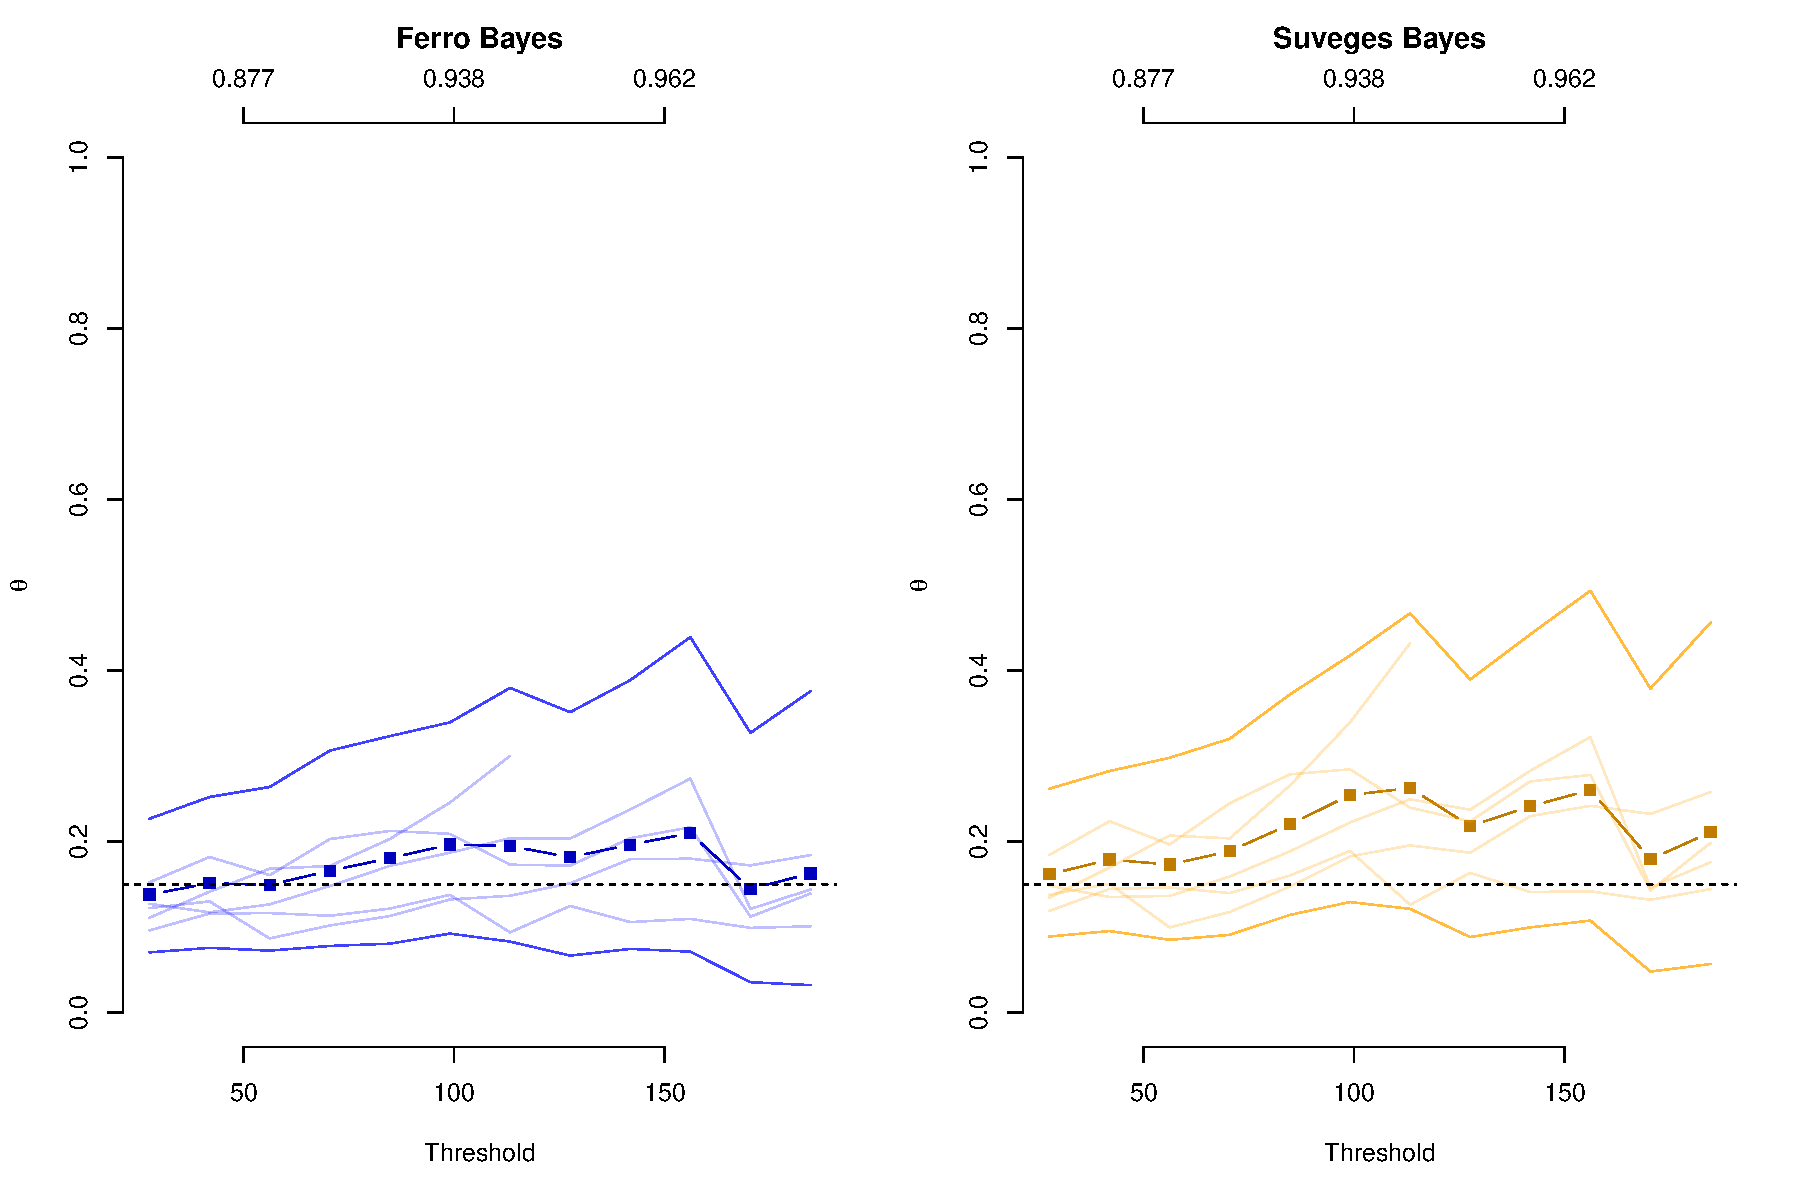
\includegraphics[width=5.5in, height=2.45in]{../extremal_comparison/figs/sim_frechet_hier_15_250_5.pdf}
\caption{$\theta=0.15$, $n=250$, $R=5$}
\end{center}
\end{figure}

\begin{figure}
\begin{center}
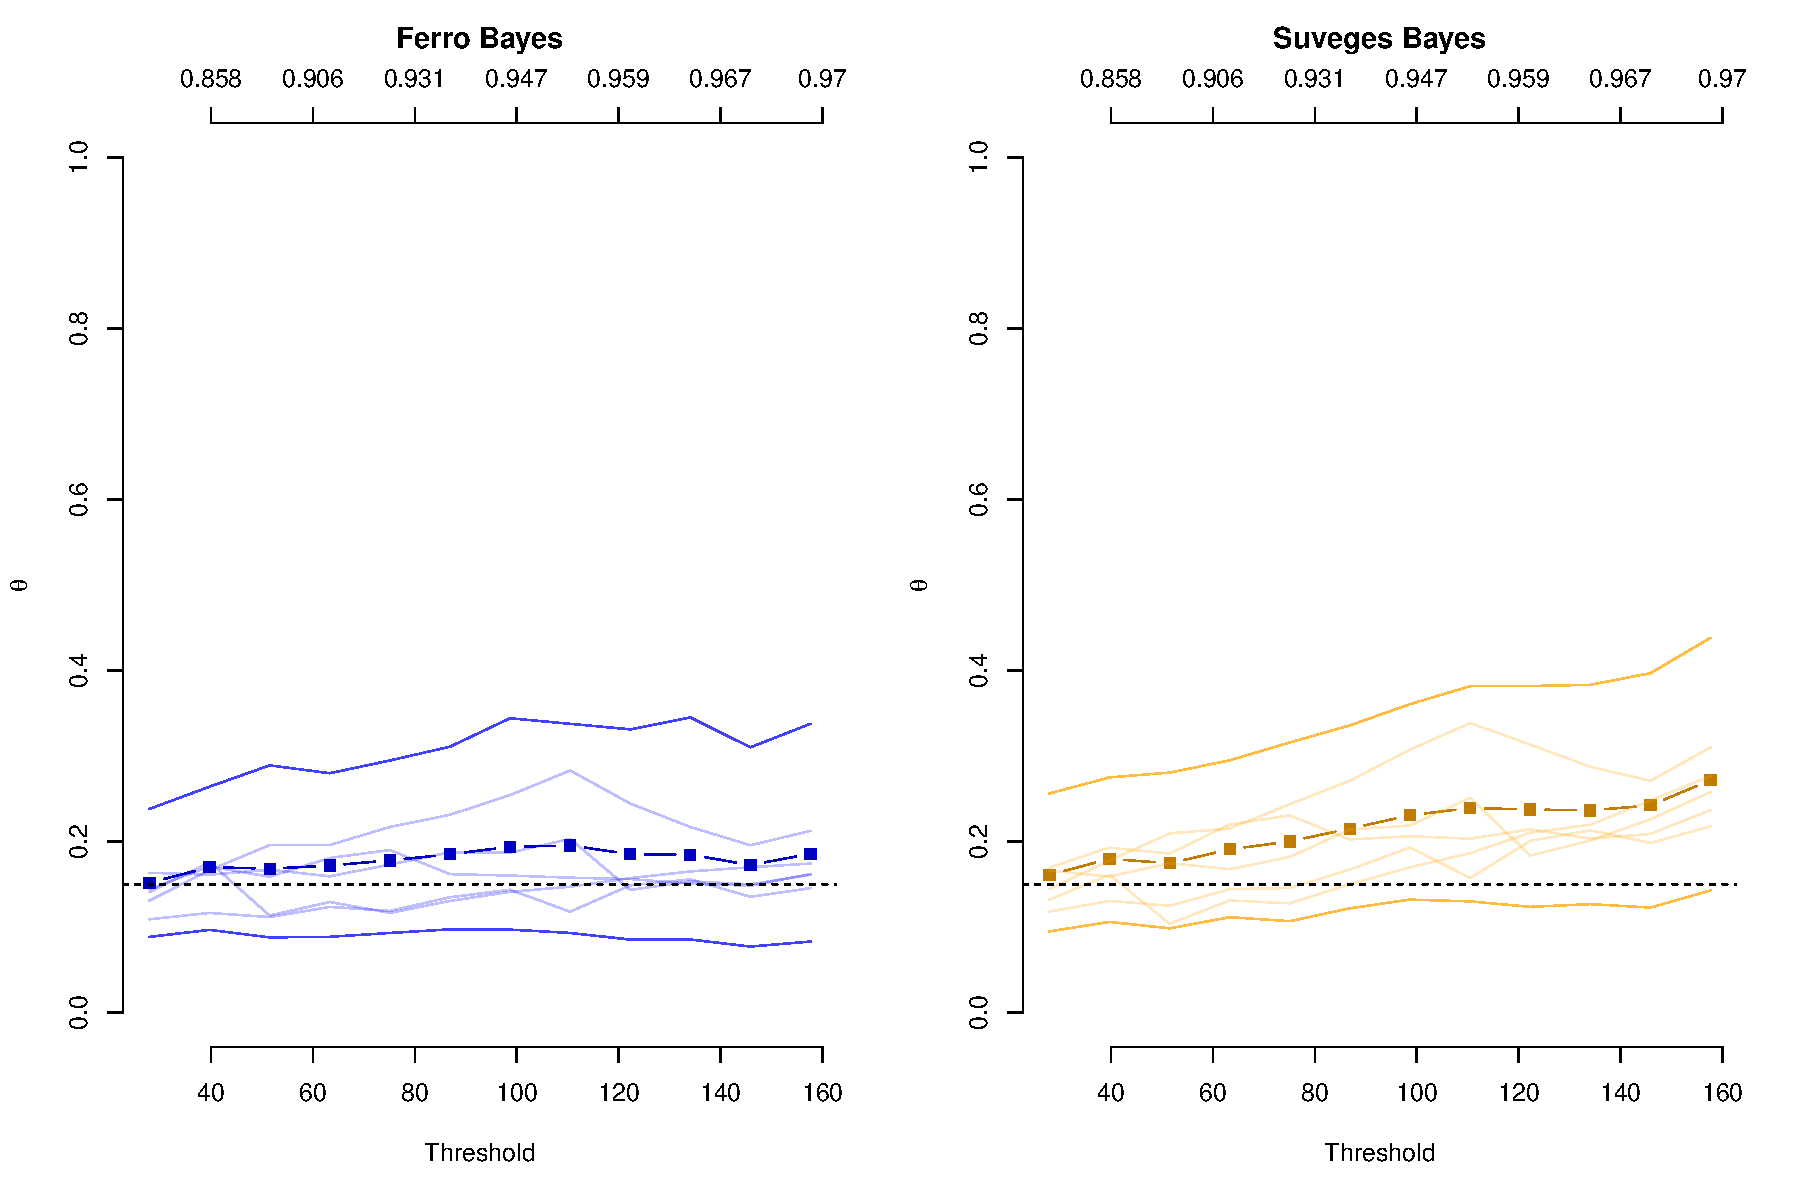
\includegraphics[width=5.5in, height=2.45in]{../extremal_comparison/figs/sim_frechet_hier_15_500_5.pdf}
\caption{$\theta=0.15$, $n=500$, $R=5$}
\end{center}
\end{figure}

\begin{figure}
\begin{center}
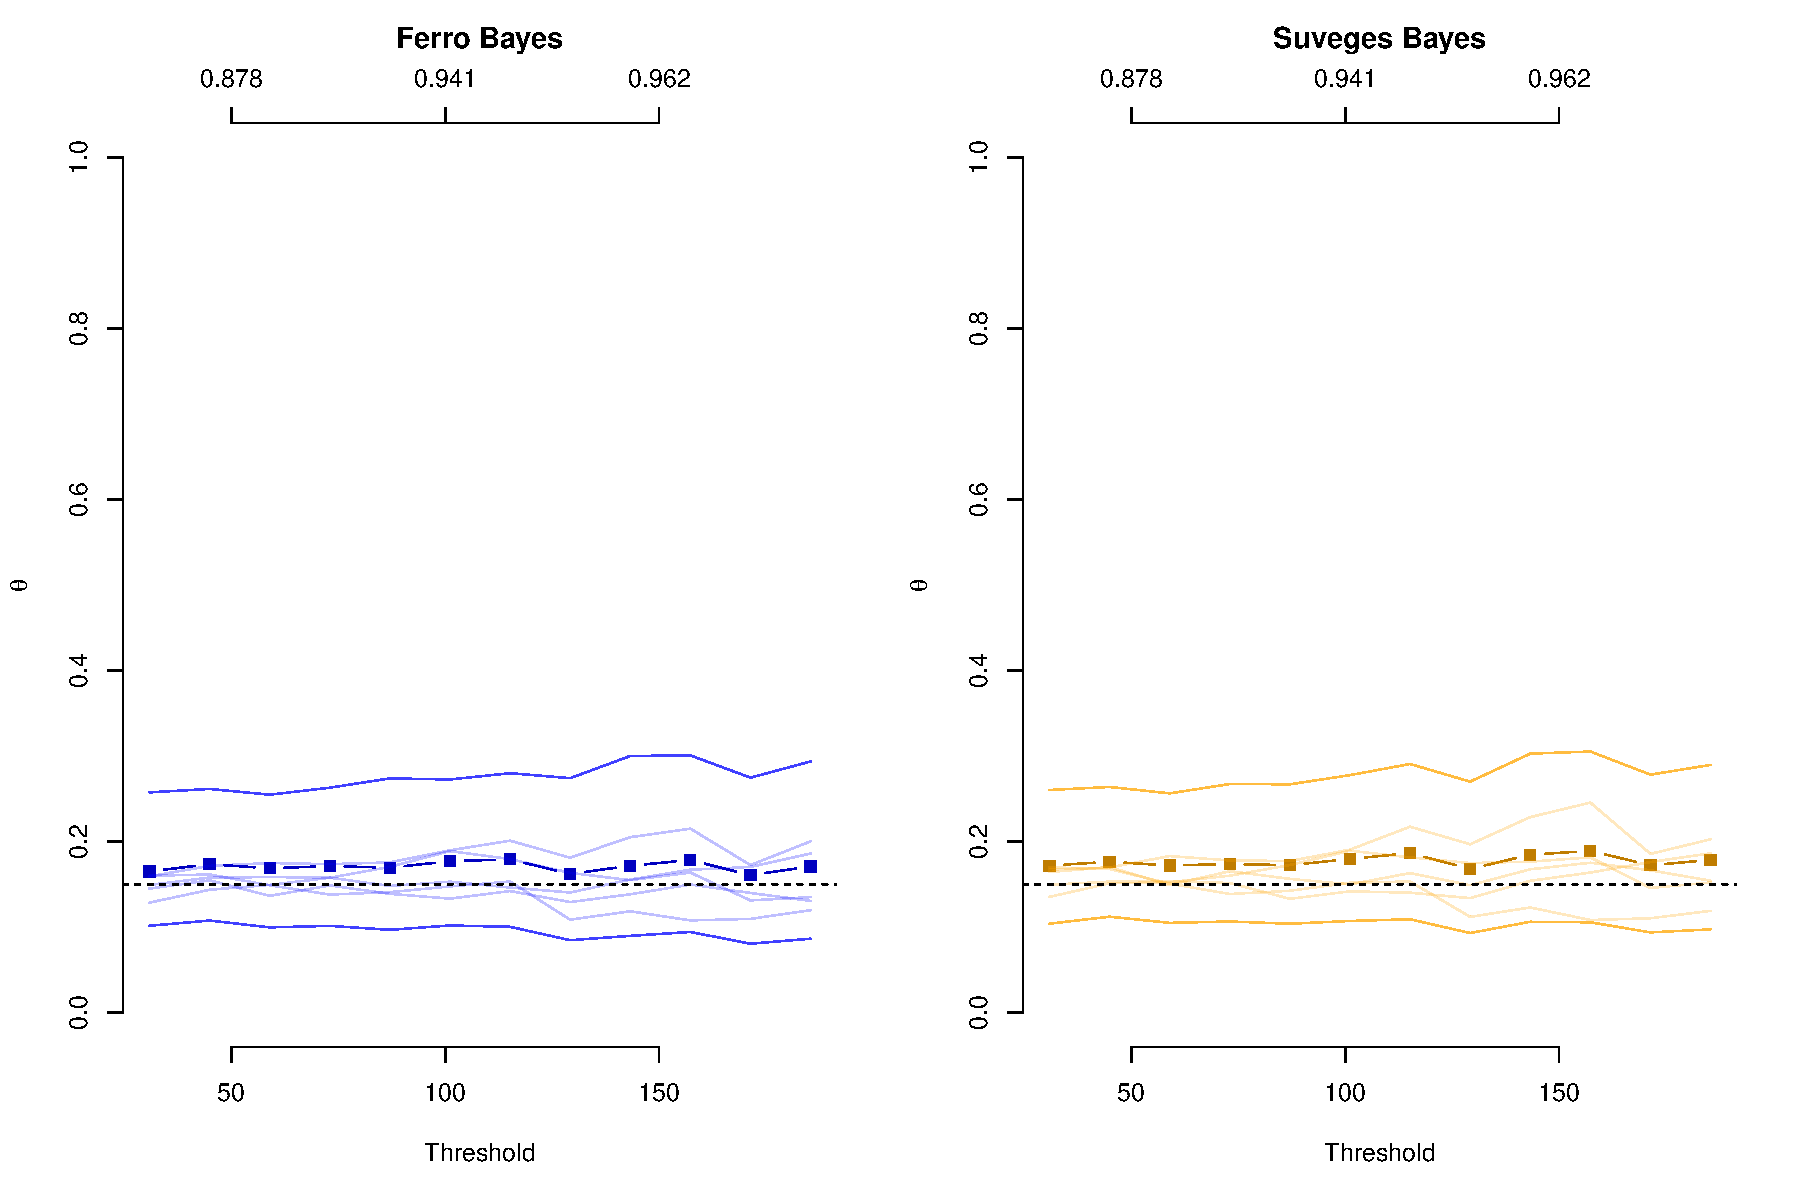
\includegraphics[width=5.5in, height=2.45in]{../extremal_comparison/figs/sim_frechet_hier_15_1000_5.pdf}
\caption{$\theta=0.15$, $n=1000$, $R=5$}
\end{center}
\end{figure}

\newpage

\begin{figure}
\begin{center}
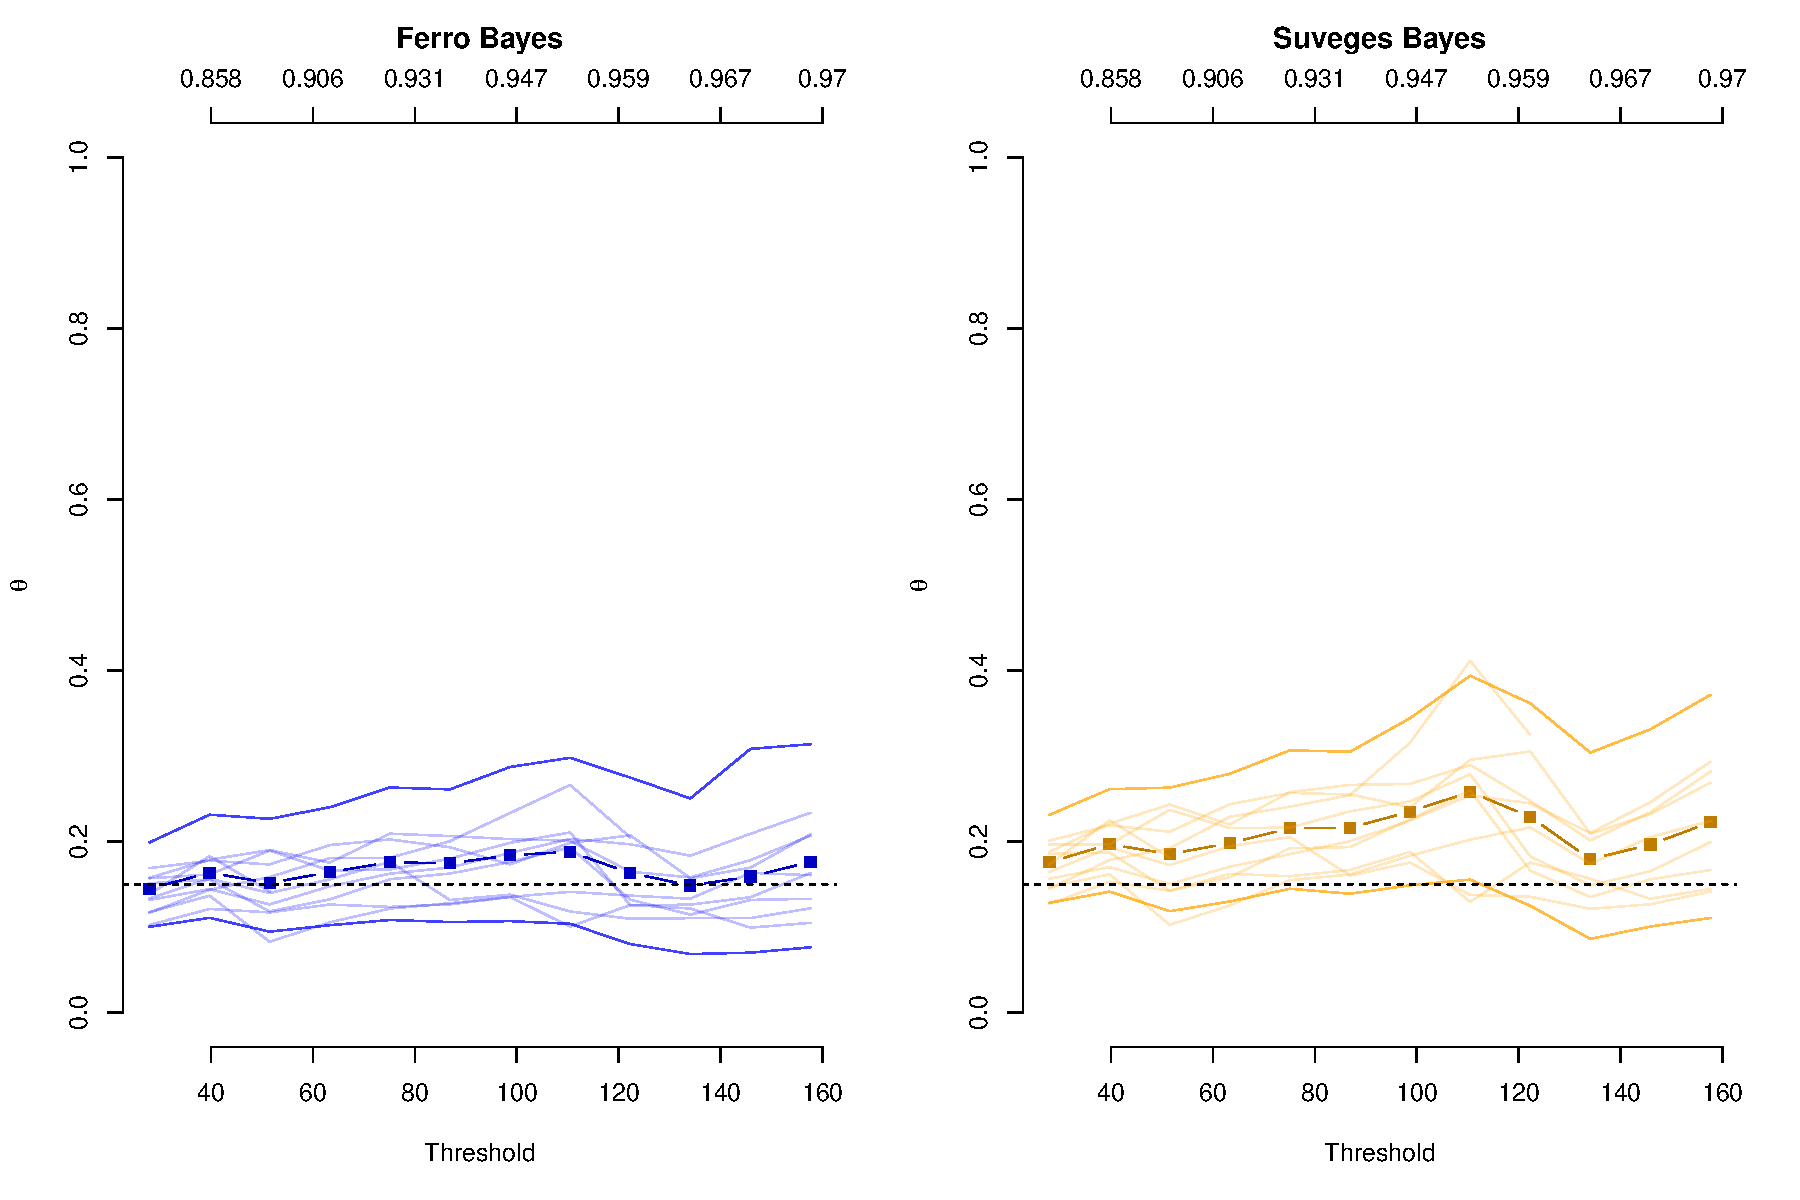
\includegraphics[width=5.5in, height=2.45in]{../extremal_comparison/figs/sim_frechet_hier_15_250_10.pdf}
\caption{$\theta=0.15$, $n=250$, $R=10$}
\end{center}
\end{figure}

\begin{figure}
\begin{center}
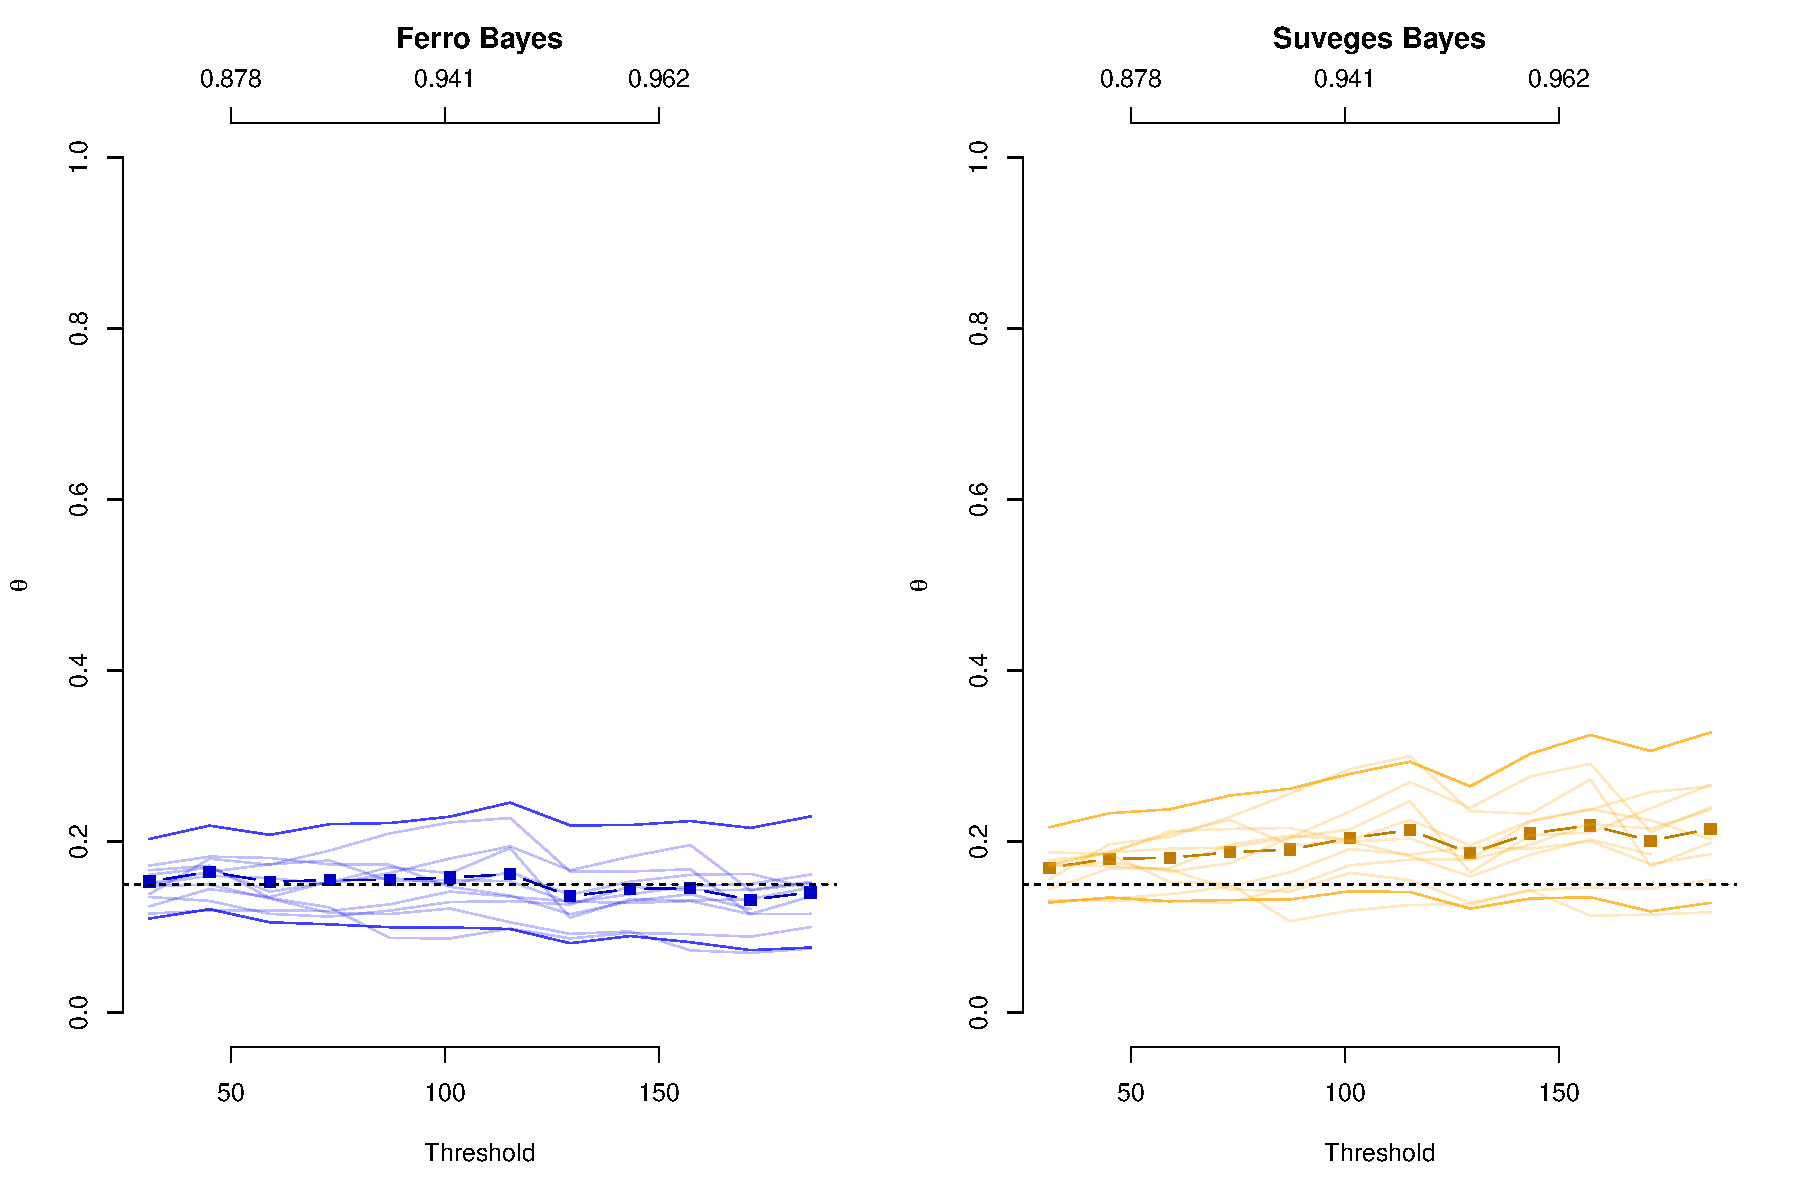
\includegraphics[width=5.5in, height=2.45in]{../extremal_comparison/figs/sim_frechet_hier_15_500_10.pdf}
\caption{$\theta=0.15$, $n=500$, $R=10$}
\end{center}
\end{figure}

\begin{figure}
\begin{center}
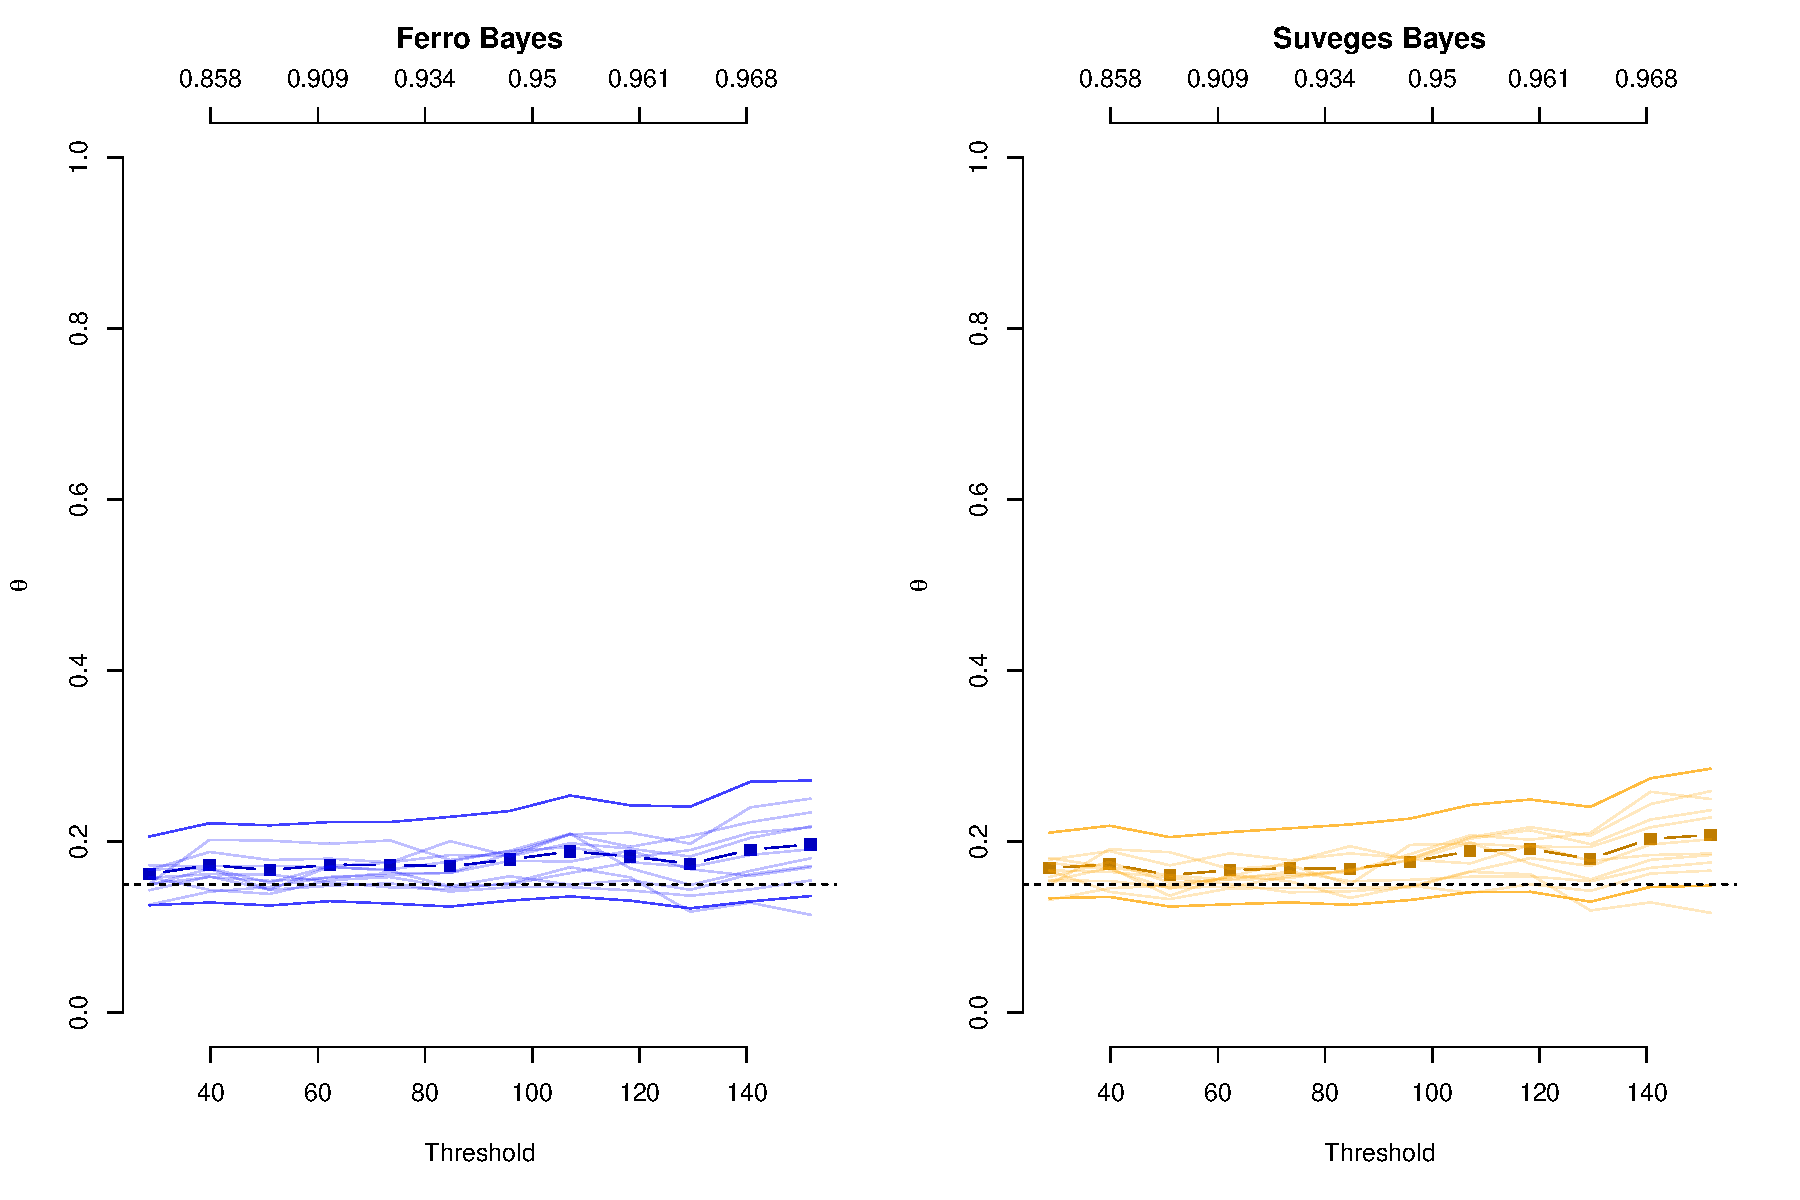
\includegraphics[width=5.5in, height=2.45in]{../extremal_comparison/figs/sim_frechet_hier_15_1000_10.pdf}
\caption{$\theta=0.15$, $n=1000$, $R=10$}
\end{center}
\end{figure}

\newpage

\begin{figure}
\begin{center}
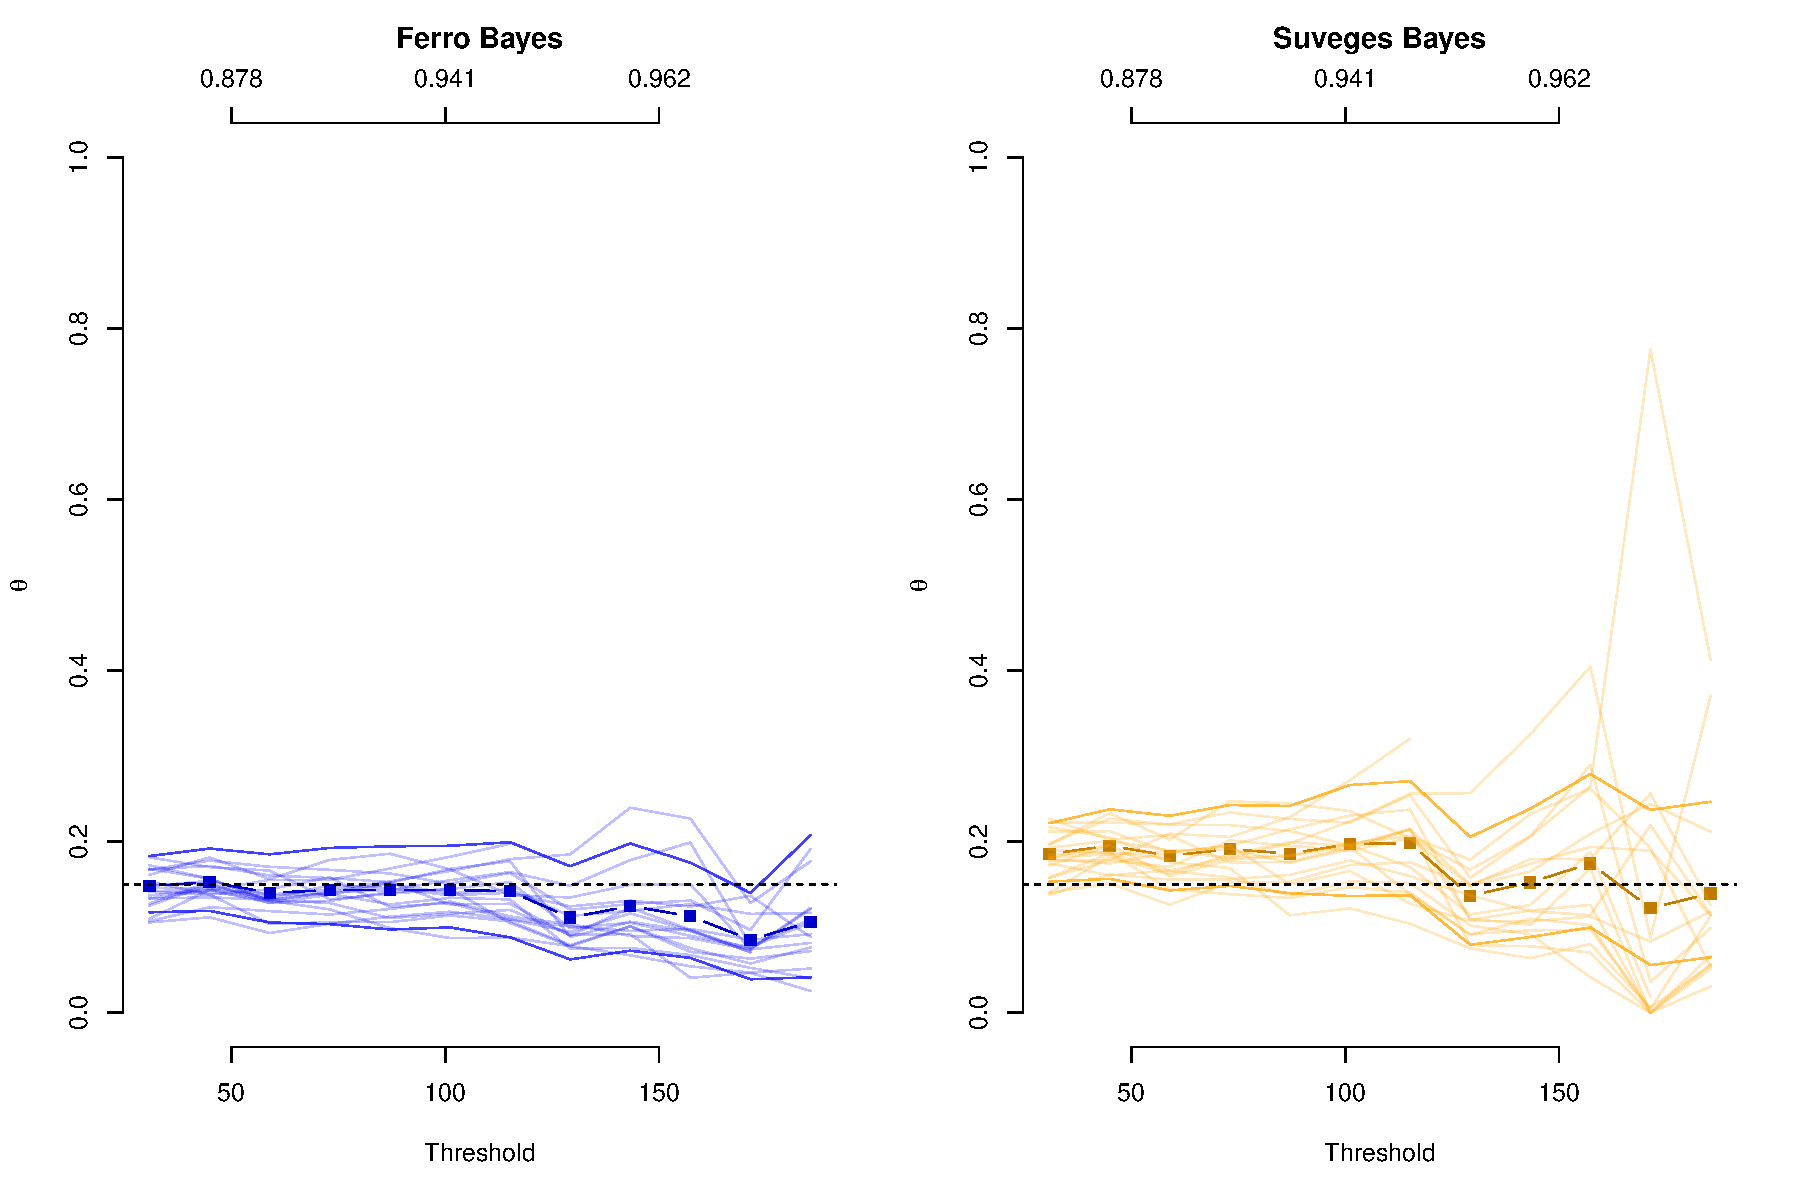
\includegraphics[width=5.5in, height=2.45in]{../extremal_comparison/figs/sim_frechet_hier_15_250_20.pdf}
\caption{$\theta=0.15$, $n=250$, $R=20$}
\end{center}
\end{figure}

\begin{figure}
\begin{center}
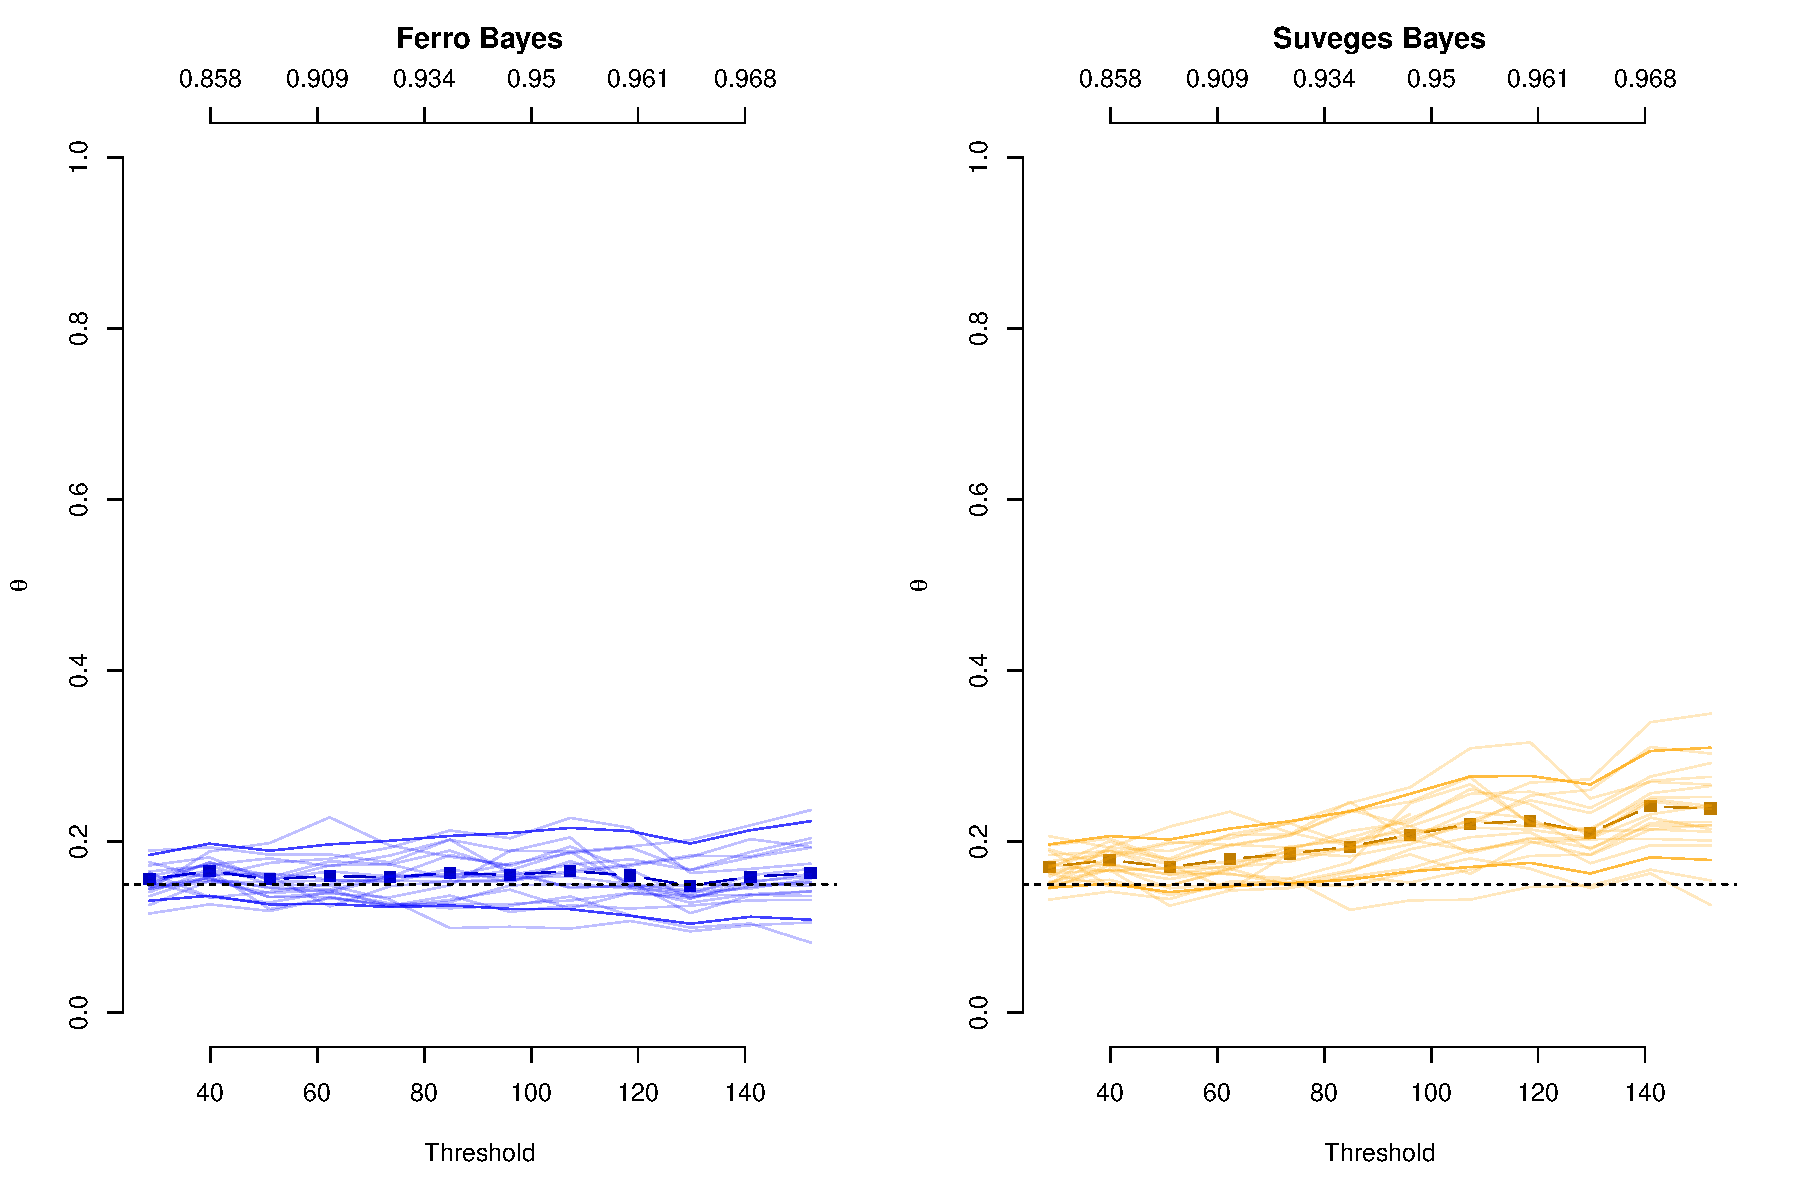
\includegraphics[width=5.5in, height=2.45in]{../extremal_comparison/figs/sim_frechet_hier_15_500_20.pdf}
\caption{$\theta=0.15$, $n=500$, $R=20$}
\end{center}
\end{figure}

\begin{figure}
\begin{center}
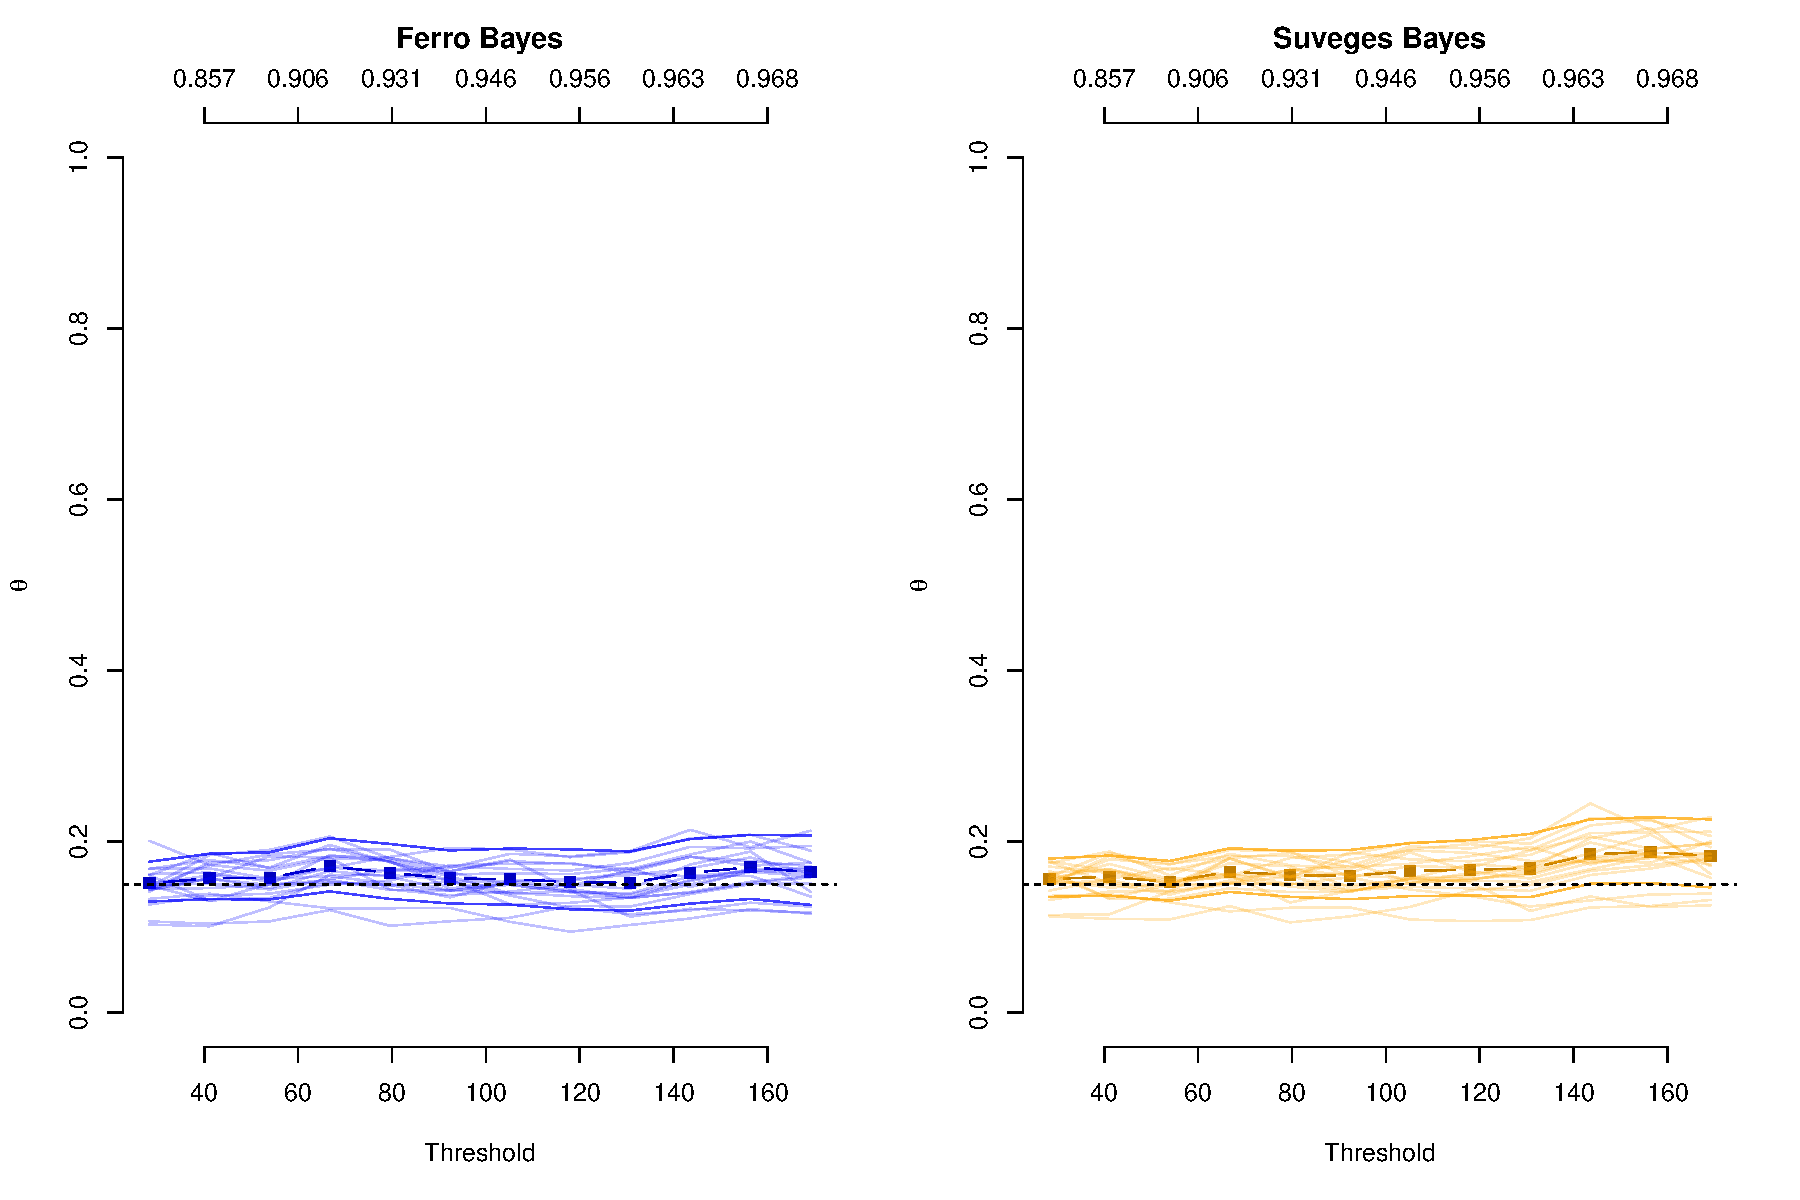
\includegraphics[width=5.5in, height=2.45in]{../extremal_comparison/figs/sim_frechet_hier_15_1000_20.pdf}
\caption{$\theta=0.15$, $n=1000$, $R=20$}
\end{center}
\end{figure}







\newpage

\begin{figure}
\begin{center}
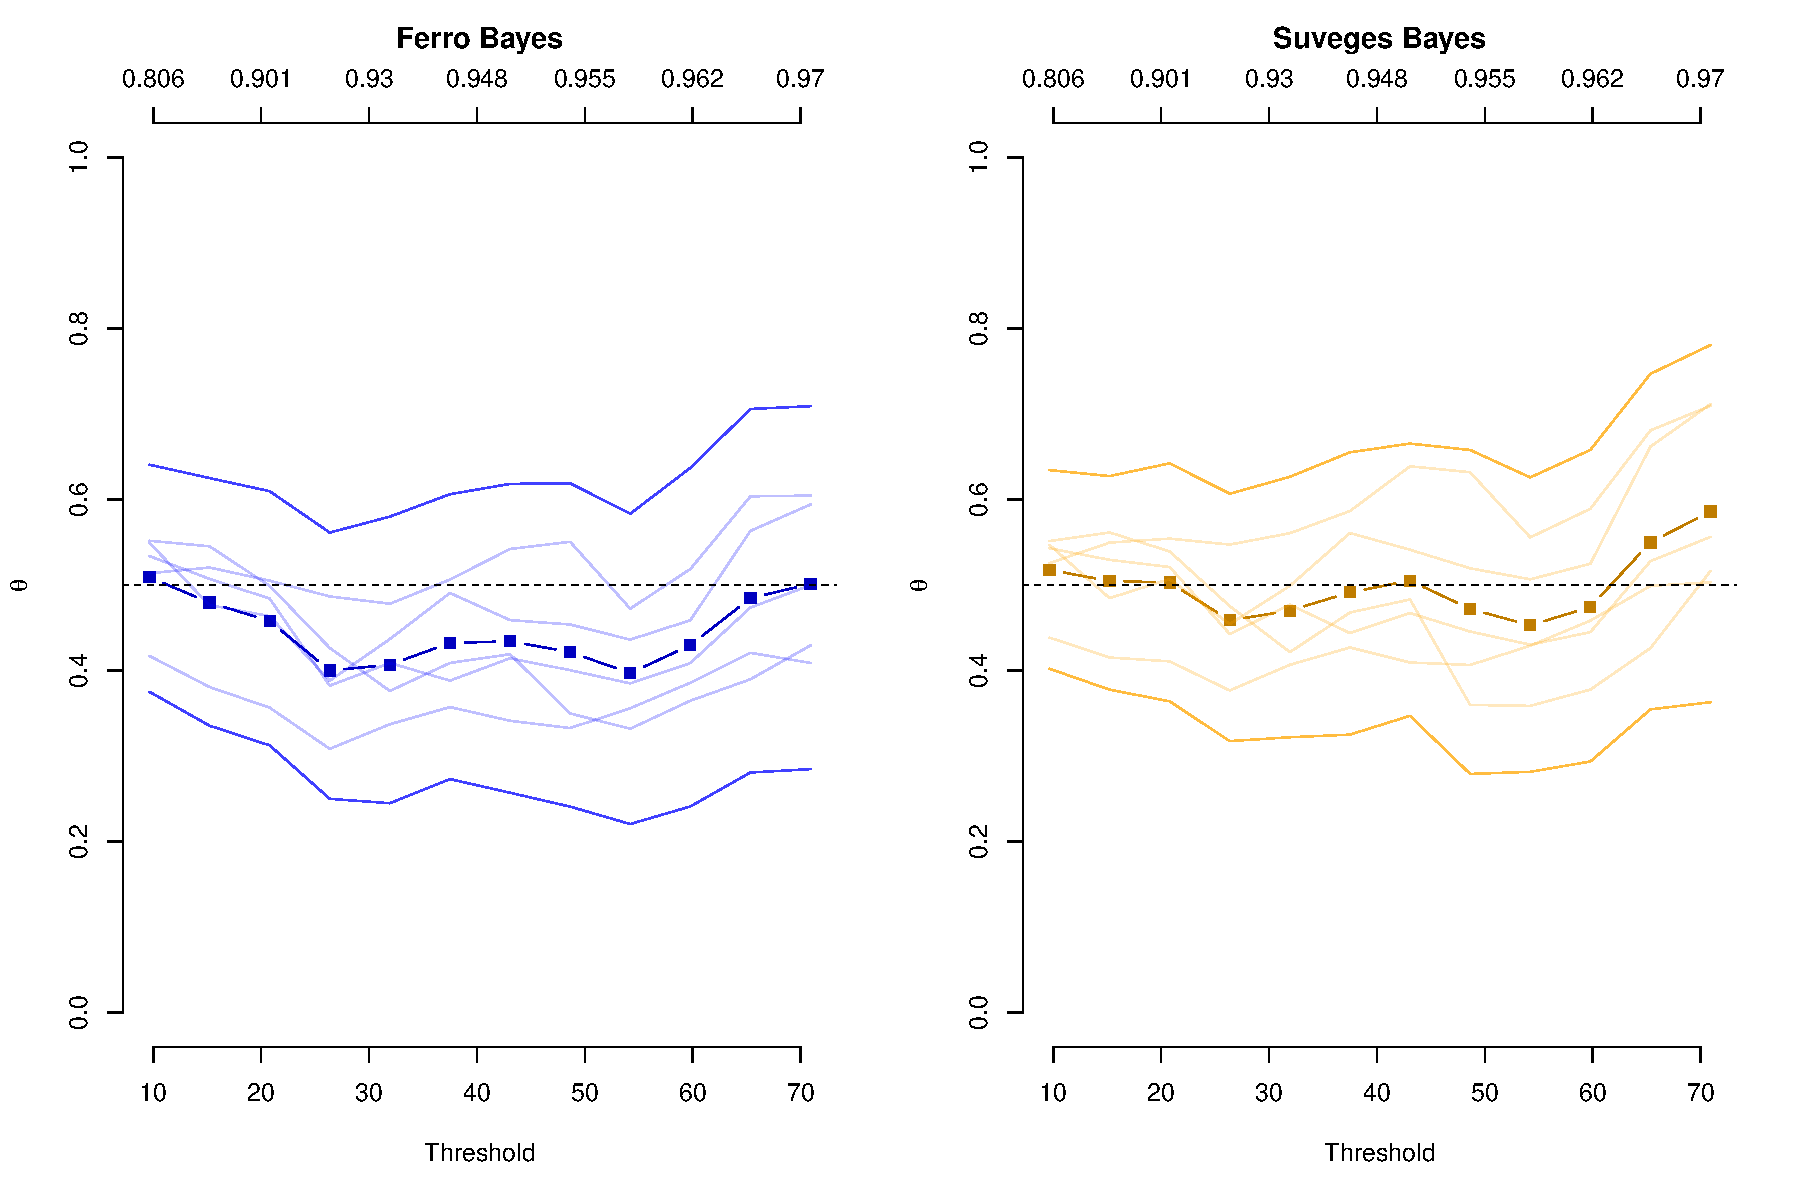
\includegraphics[width=5.5in, height=2.45in]{../extremal_comparison/figs/sim_frechet_hier_50_250_5.pdf}
\caption{$\theta=0.50$, $n=250$, $R=5$}
\end{center}
\end{figure}

\begin{figure}
\begin{center}
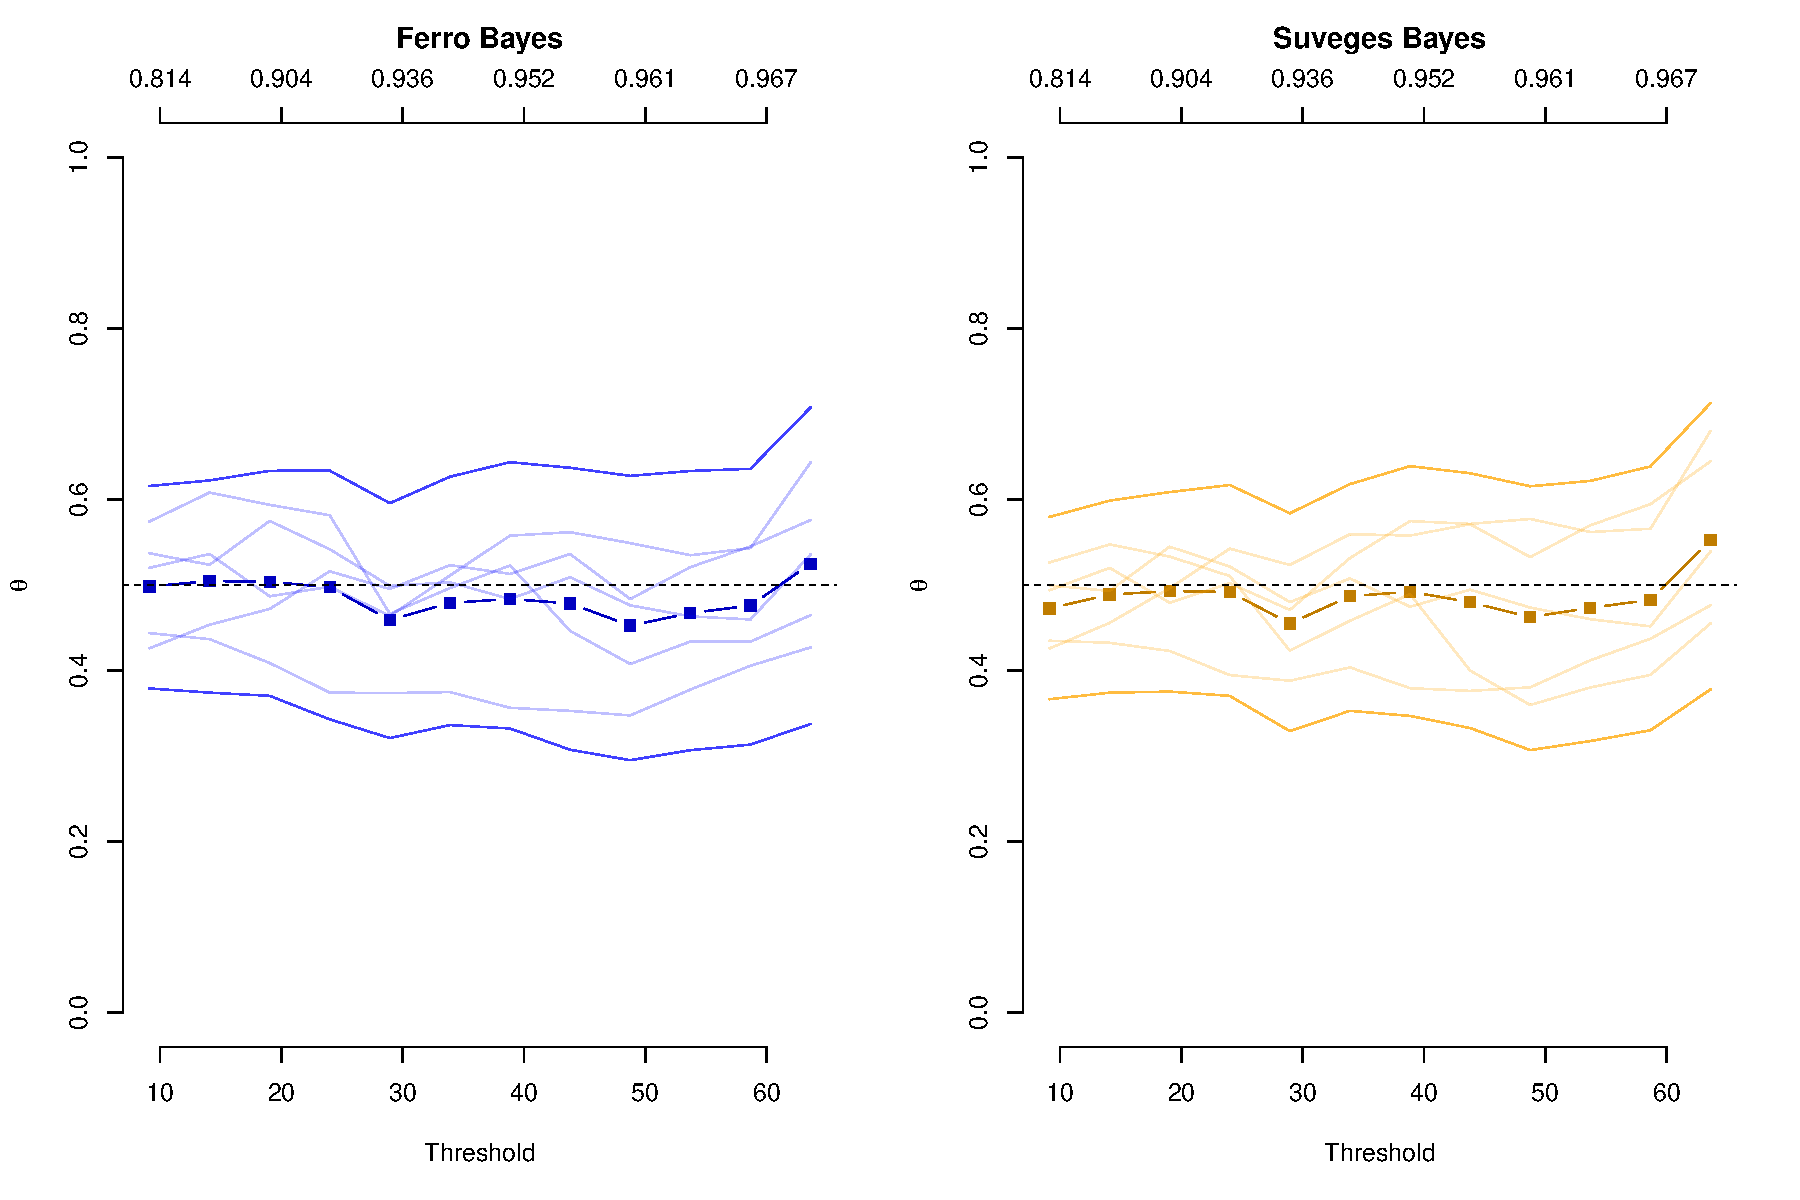
\includegraphics[width=5.5in, height=2.45in]{../extremal_comparison/figs/sim_frechet_hier_50_500_5.pdf}
\caption{$\theta=0.50$, $n=500$, $R=5$}
\end{center}
\end{figure}

\begin{figure}
\begin{center}
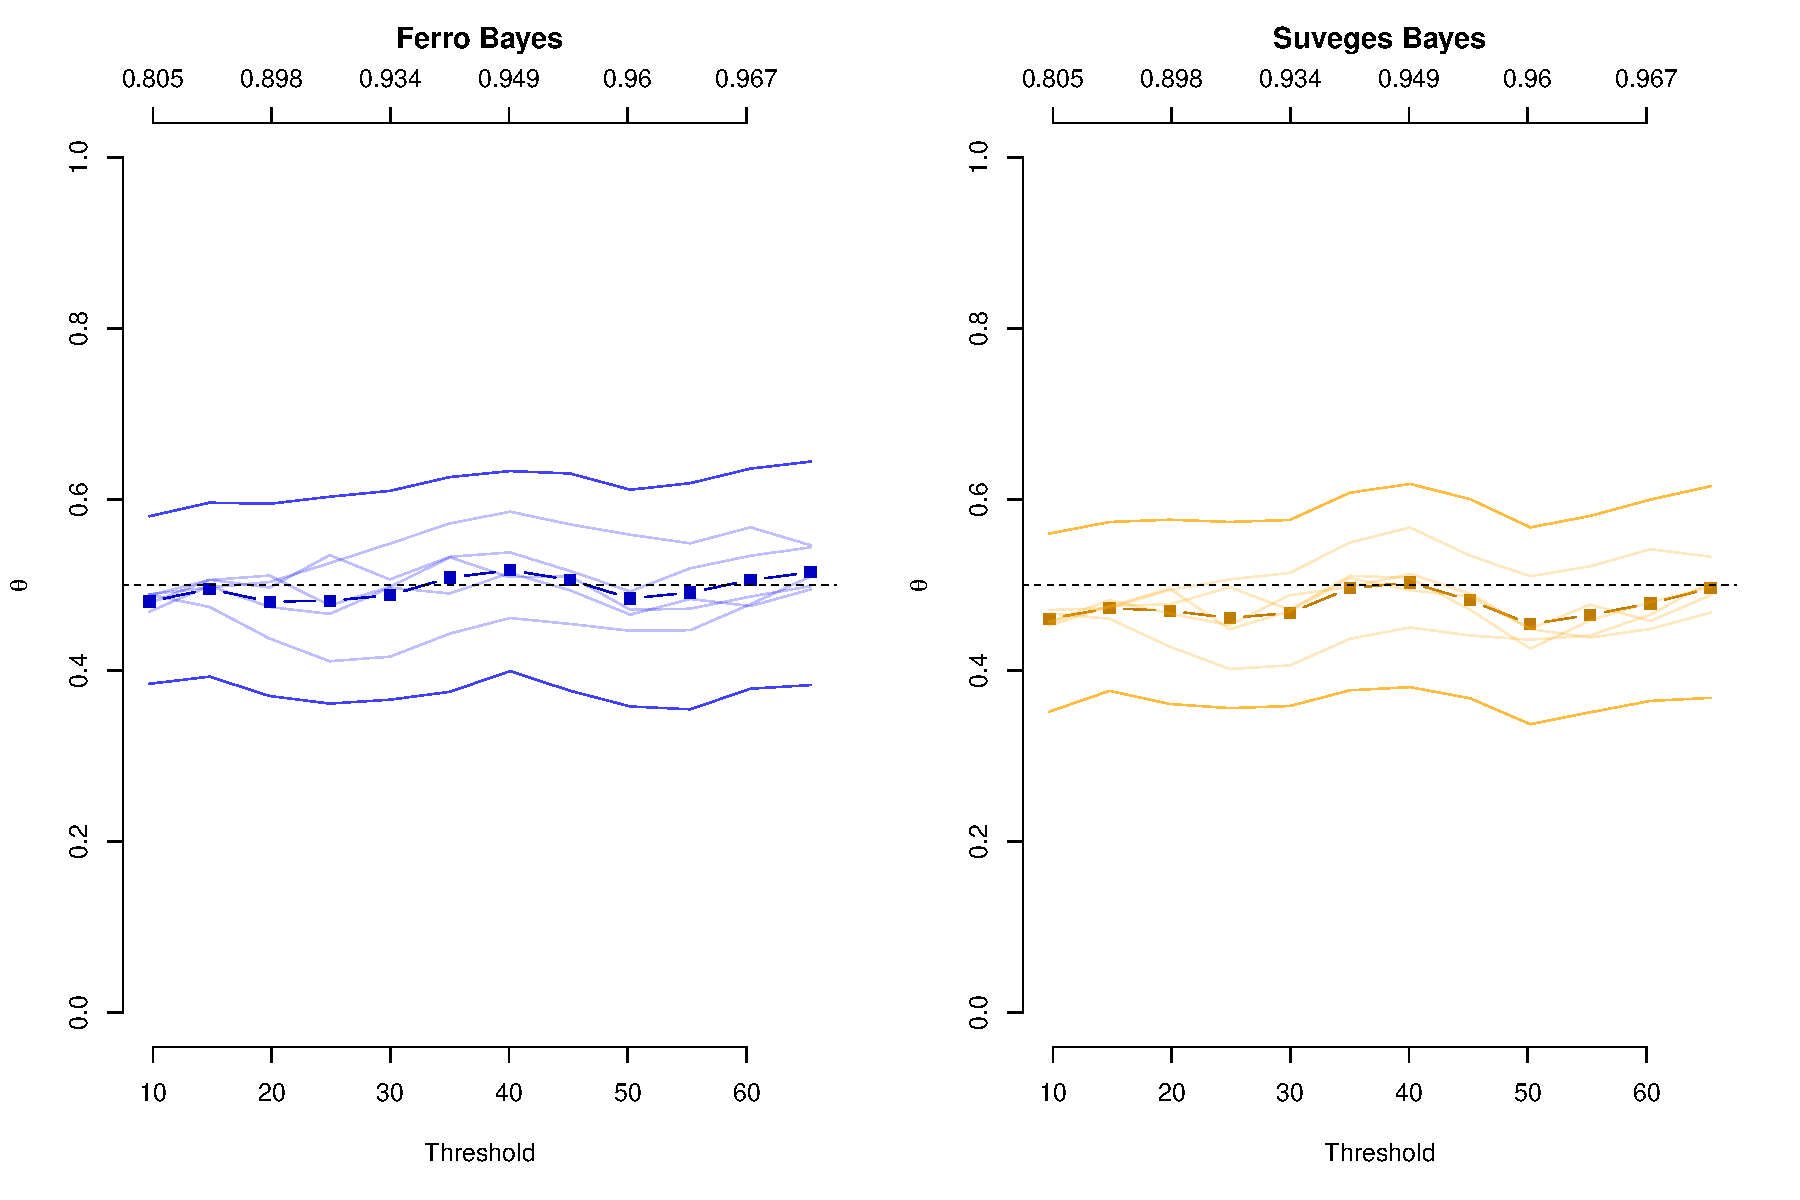
\includegraphics[width=5.5in, height=2.45in]{../extremal_comparison/figs/sim_frechet_hier_50_1000_5.pdf}
\caption{$\theta=0.50$, $n=1000$, $R=5$}
\end{center}
\end{figure}

\newpage

\begin{figure}
\begin{center}
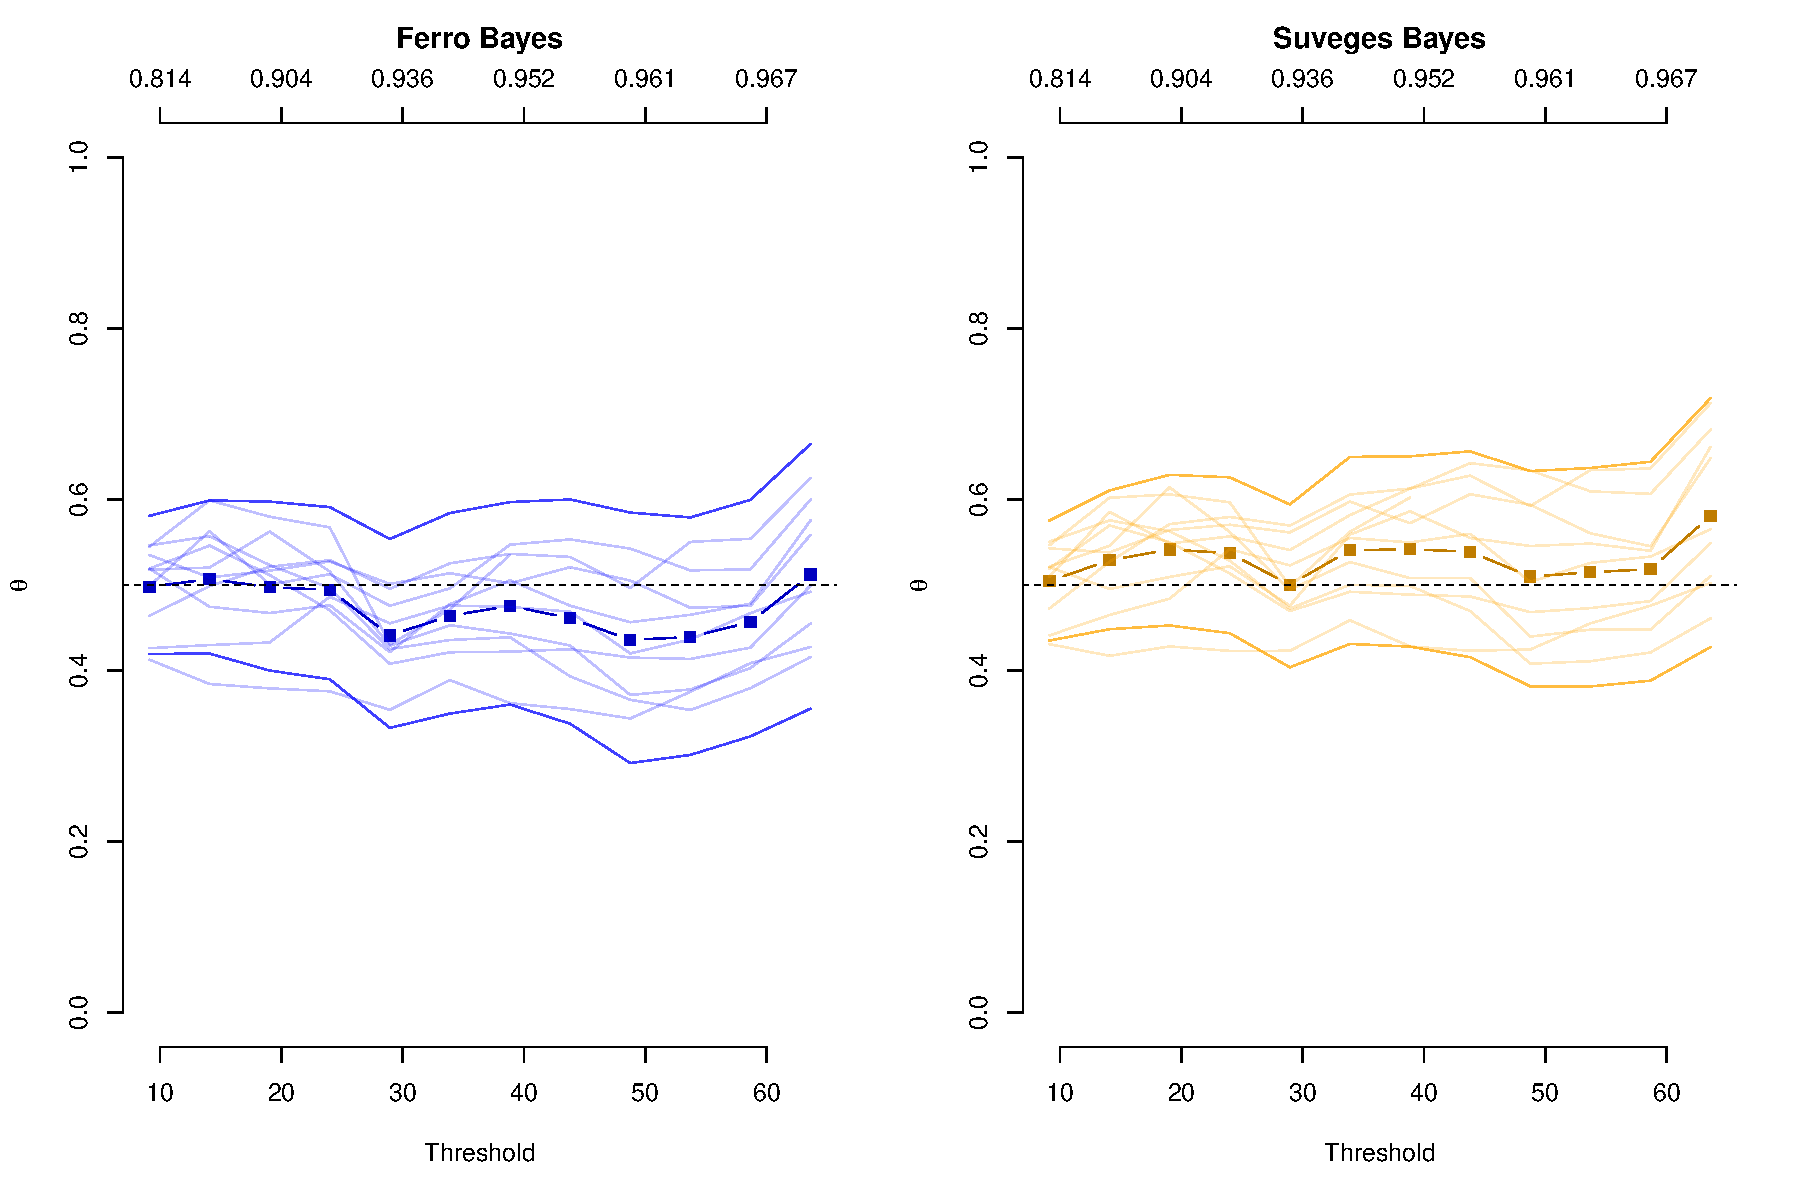
\includegraphics[width=5.5in, height=2.45in]{../extremal_comparison/figs/sim_frechet_hier_50_250_10.pdf}
\caption{$\theta=0.50$, $n=250$, $R=10$}
\end{center}
\end{figure}

\begin{figure}
\begin{center}
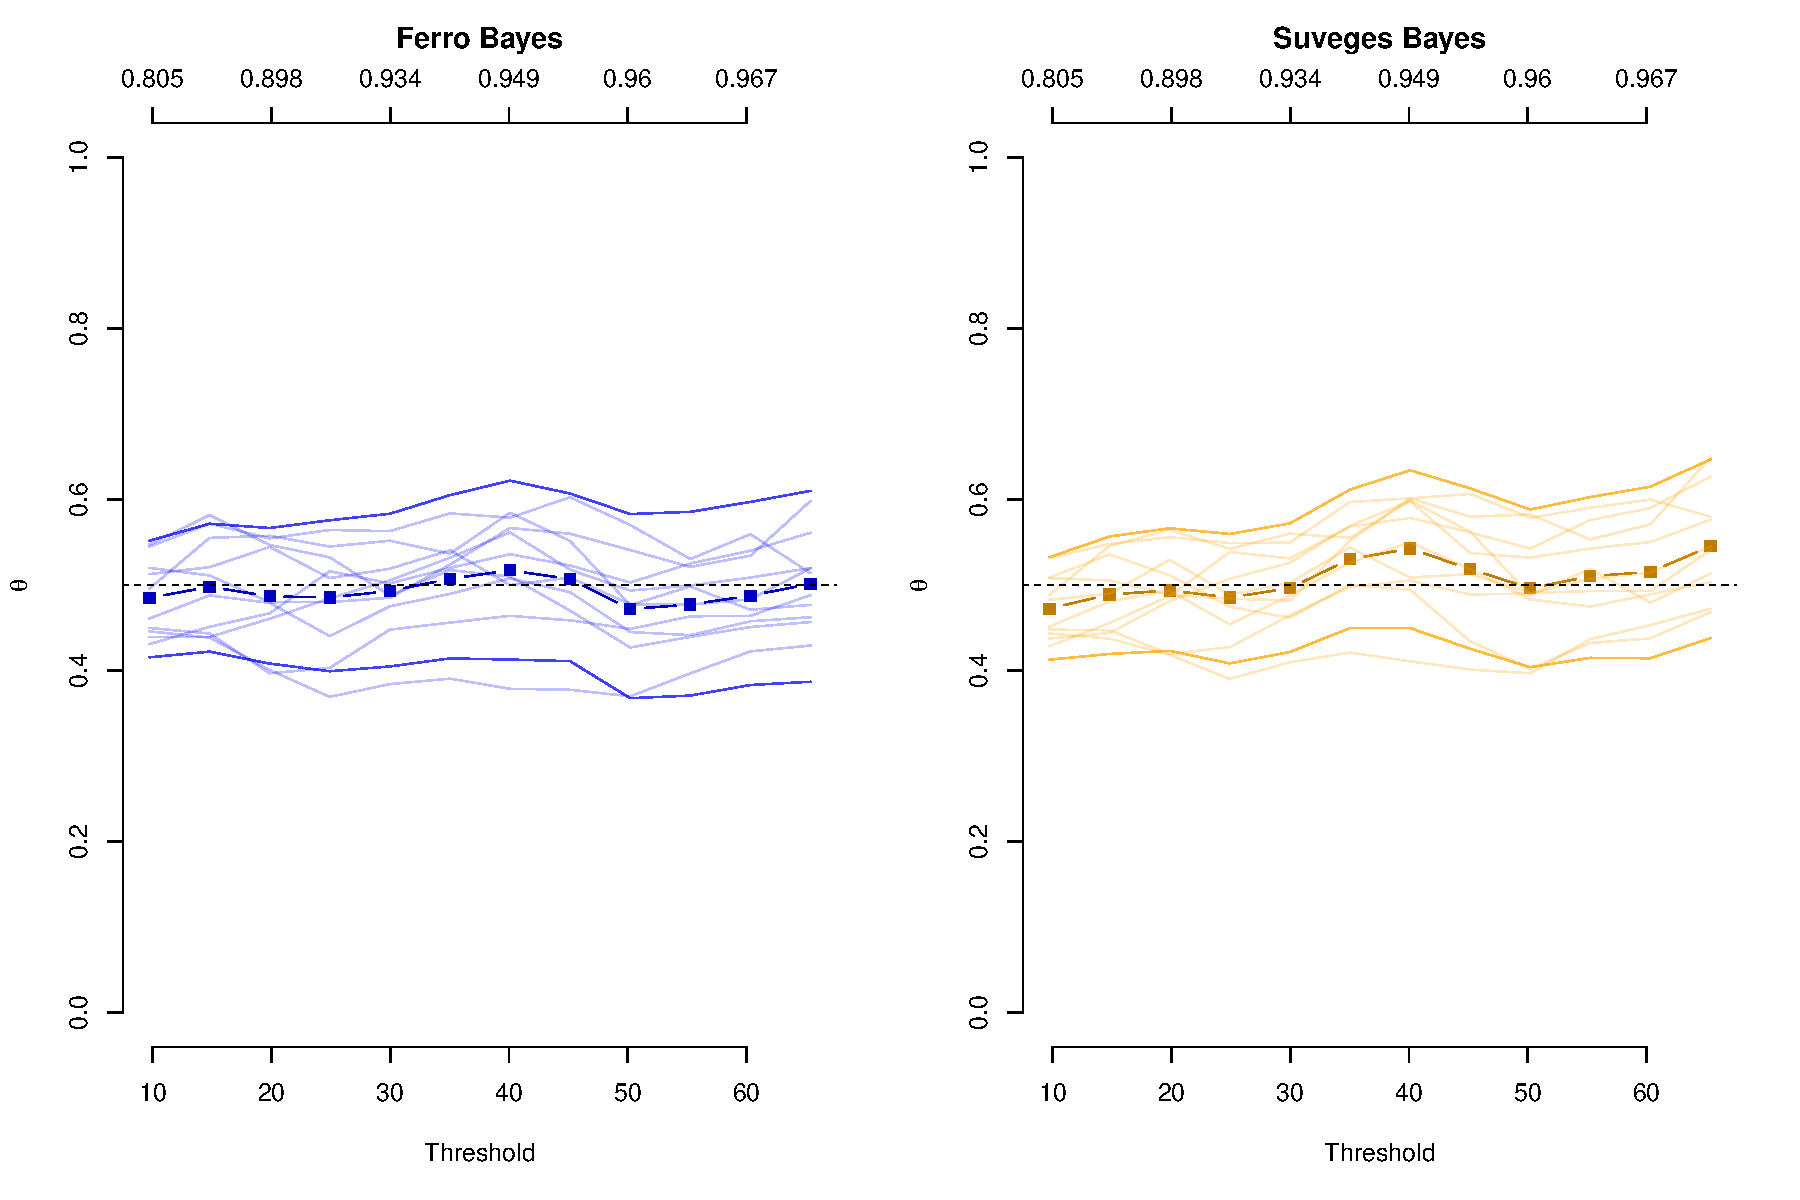
\includegraphics[width=5.5in, height=2.45in]{../extremal_comparison/figs/sim_frechet_hier_50_500_10.pdf}
\caption{$\theta=0.50$, $n=500$, $R=10$}
\end{center}
\end{figure}

\begin{figure}
\begin{center}
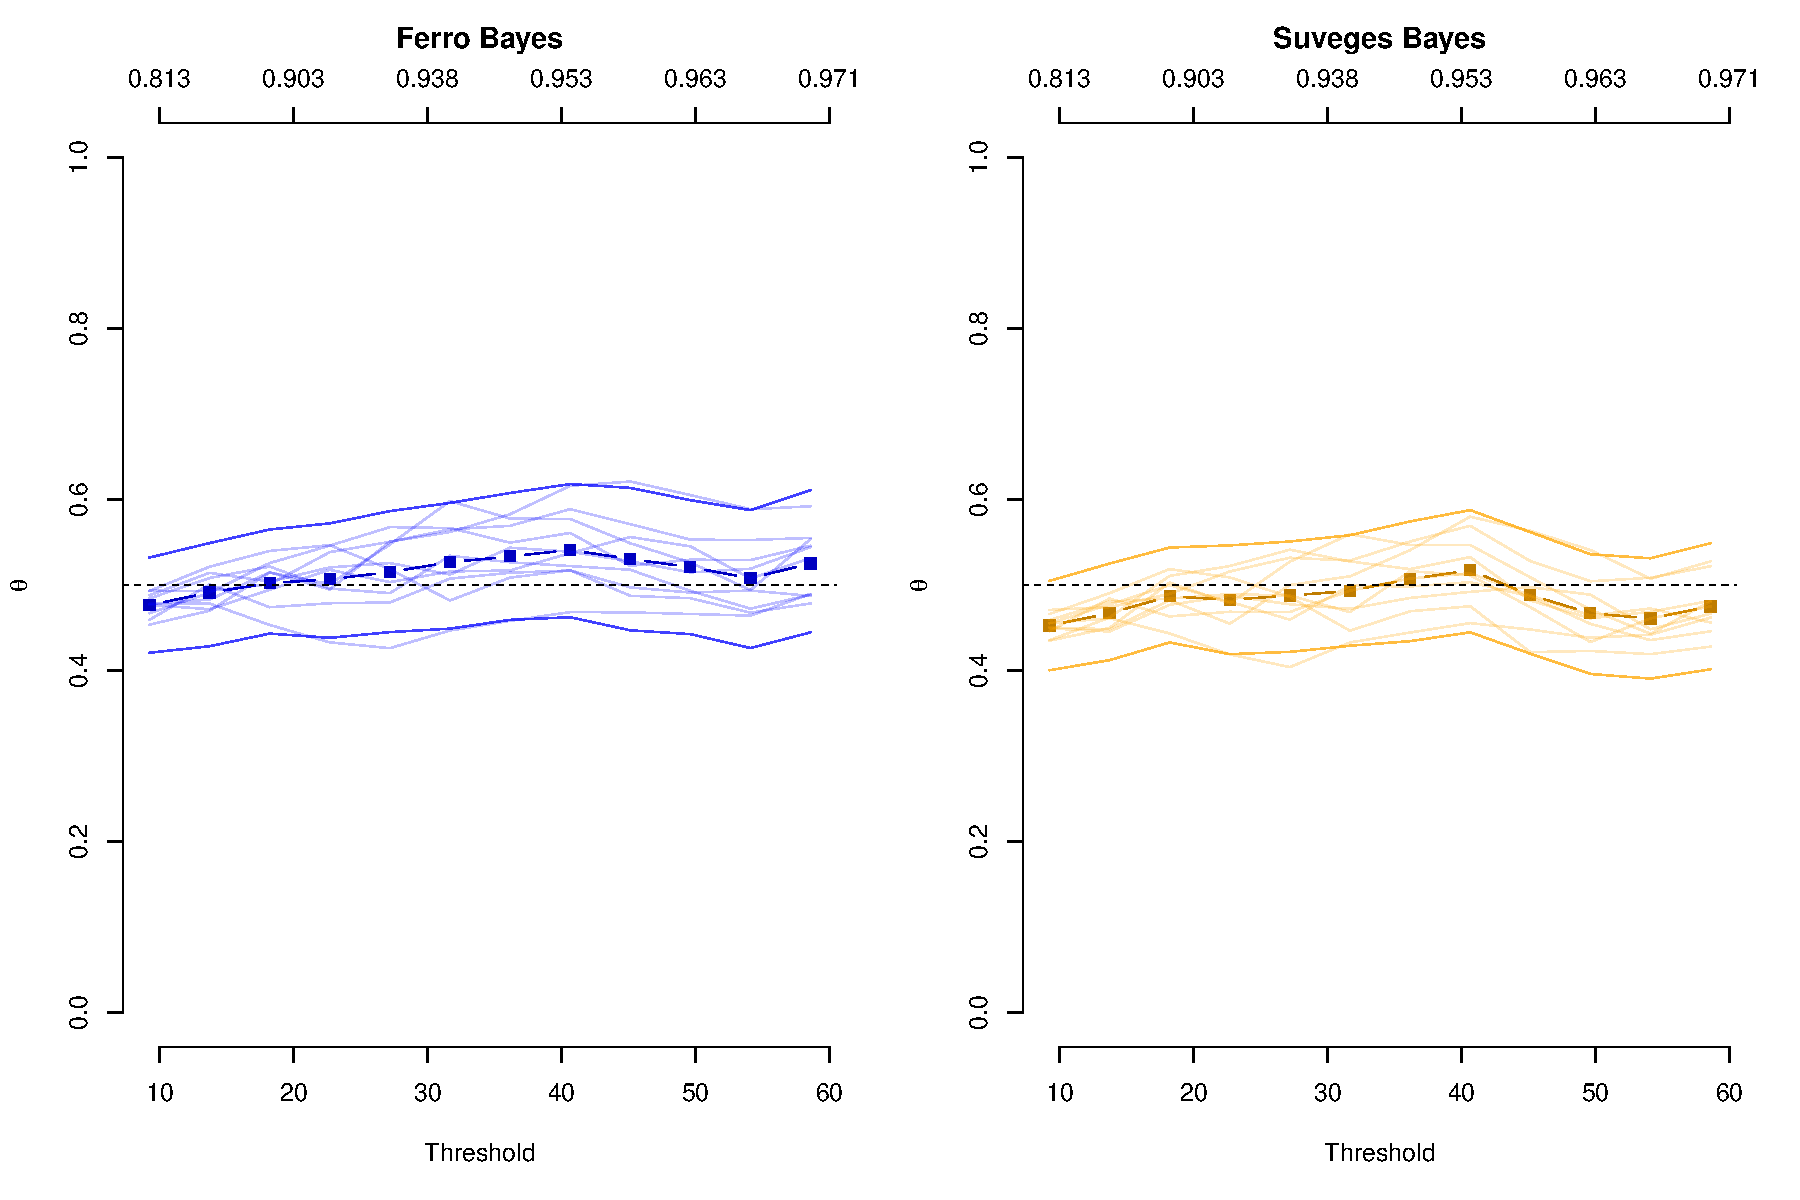
\includegraphics[width=5.5in, height=2.45in]{../extremal_comparison/figs/sim_frechet_hier_50_1000_10.pdf}
\caption{$\theta=0.50$, $n=1000$, $R=10$}
\end{center}
\end{figure}

\newpage

\begin{figure}
\begin{center}
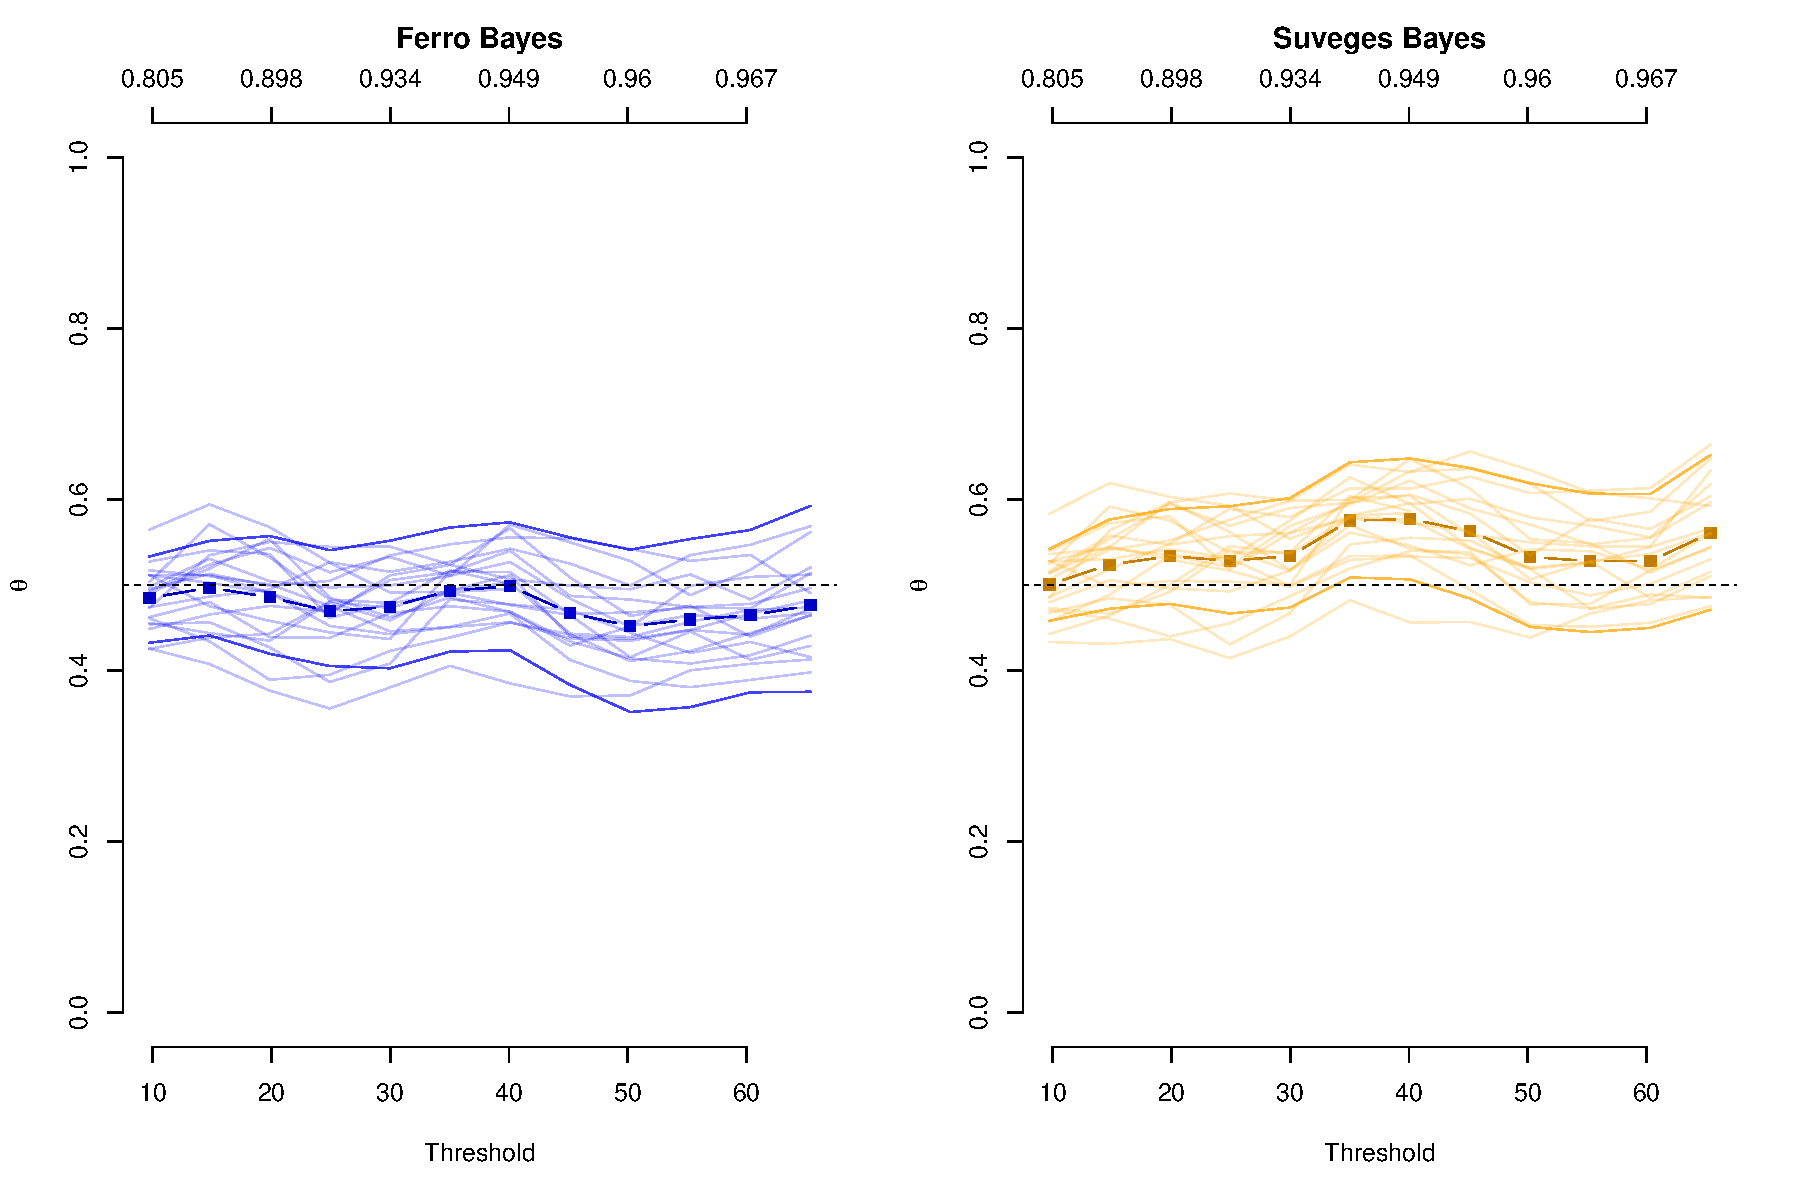
\includegraphics[width=5.5in, height=2.45in]{../extremal_comparison/figs/sim_frechet_hier_50_250_20.pdf}
\caption{$\theta=0.50$, $n=250$, $R=20$}
\end{center}
\end{figure}

\begin{figure}
\begin{center}
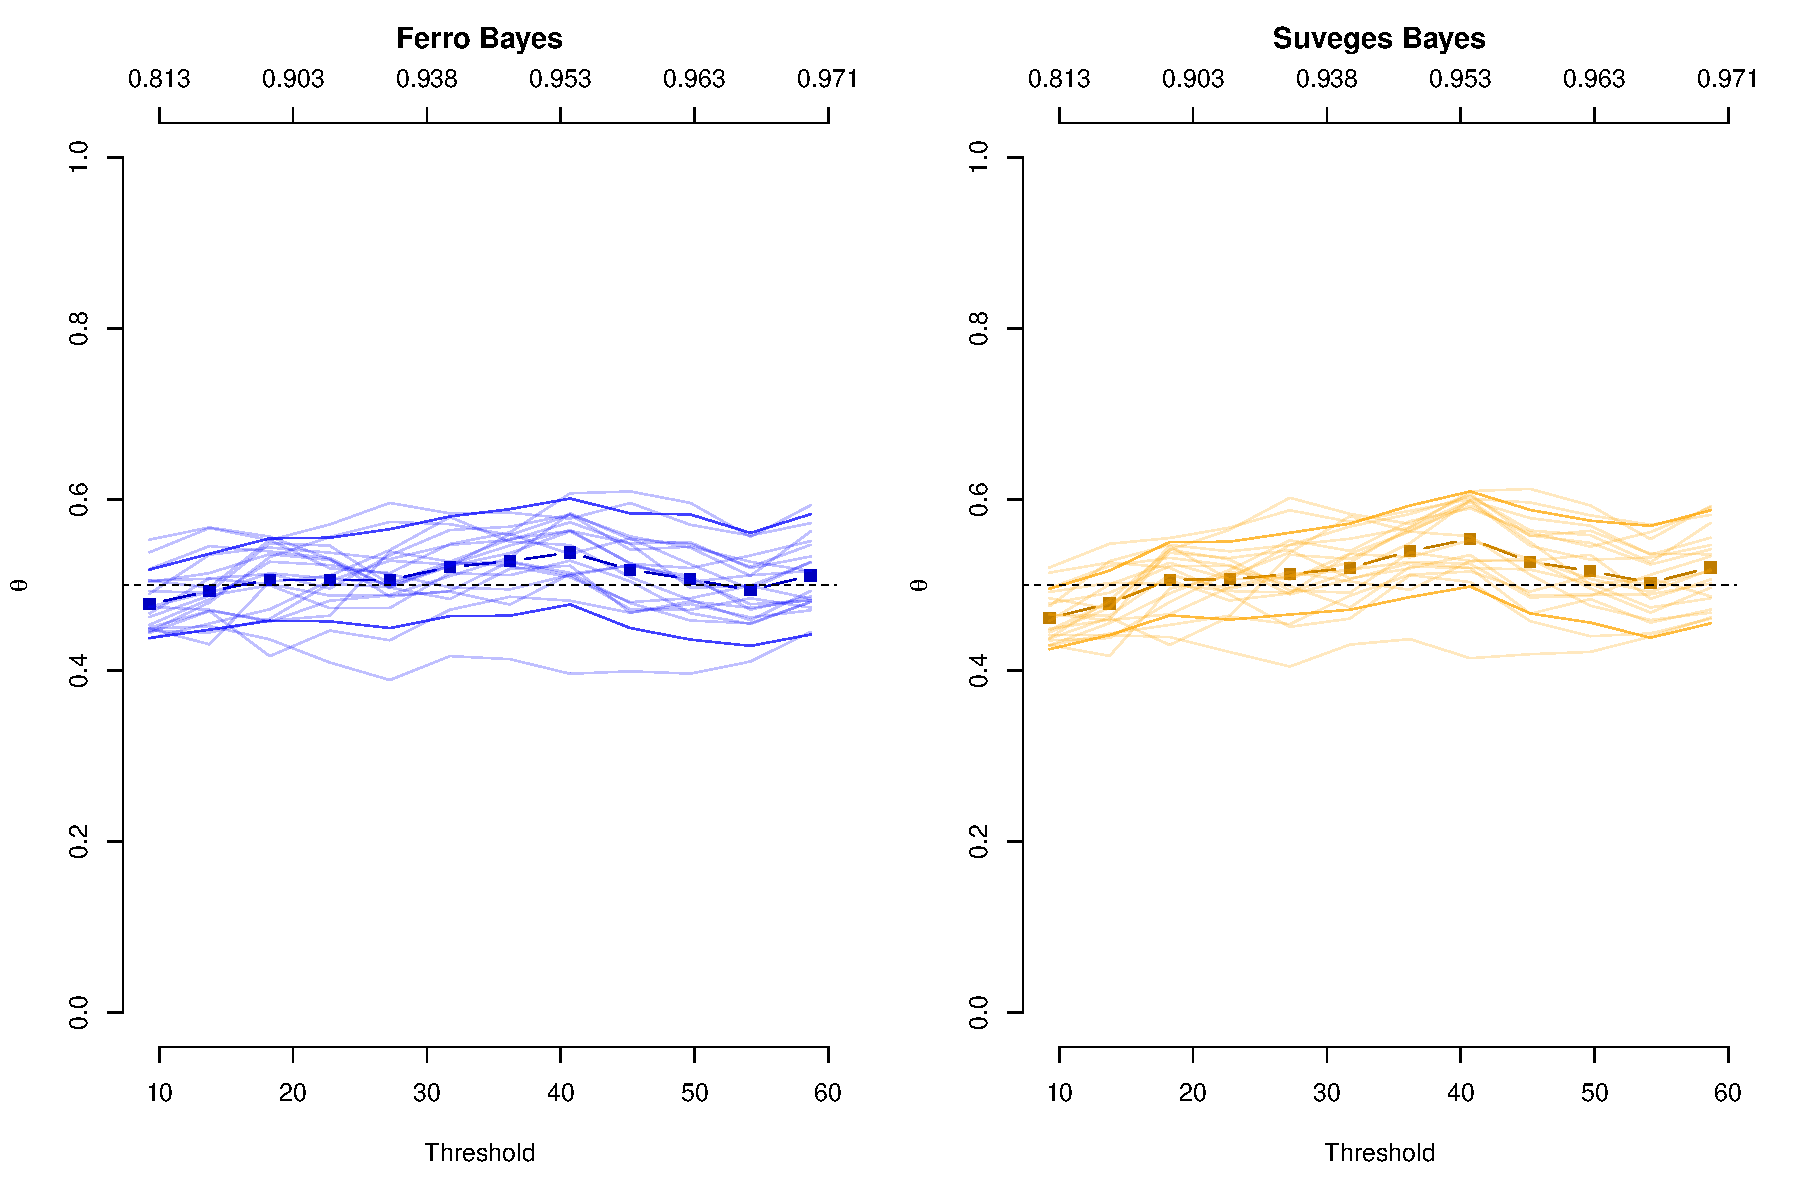
\includegraphics[width=5.5in, height=2.45in]{../extremal_comparison/figs/sim_frechet_hier_50_500_20.pdf}
\caption{$\theta=0.50$, $n=500$, $R=20$}
\end{center}
\end{figure}

\begin{figure}
\begin{center}
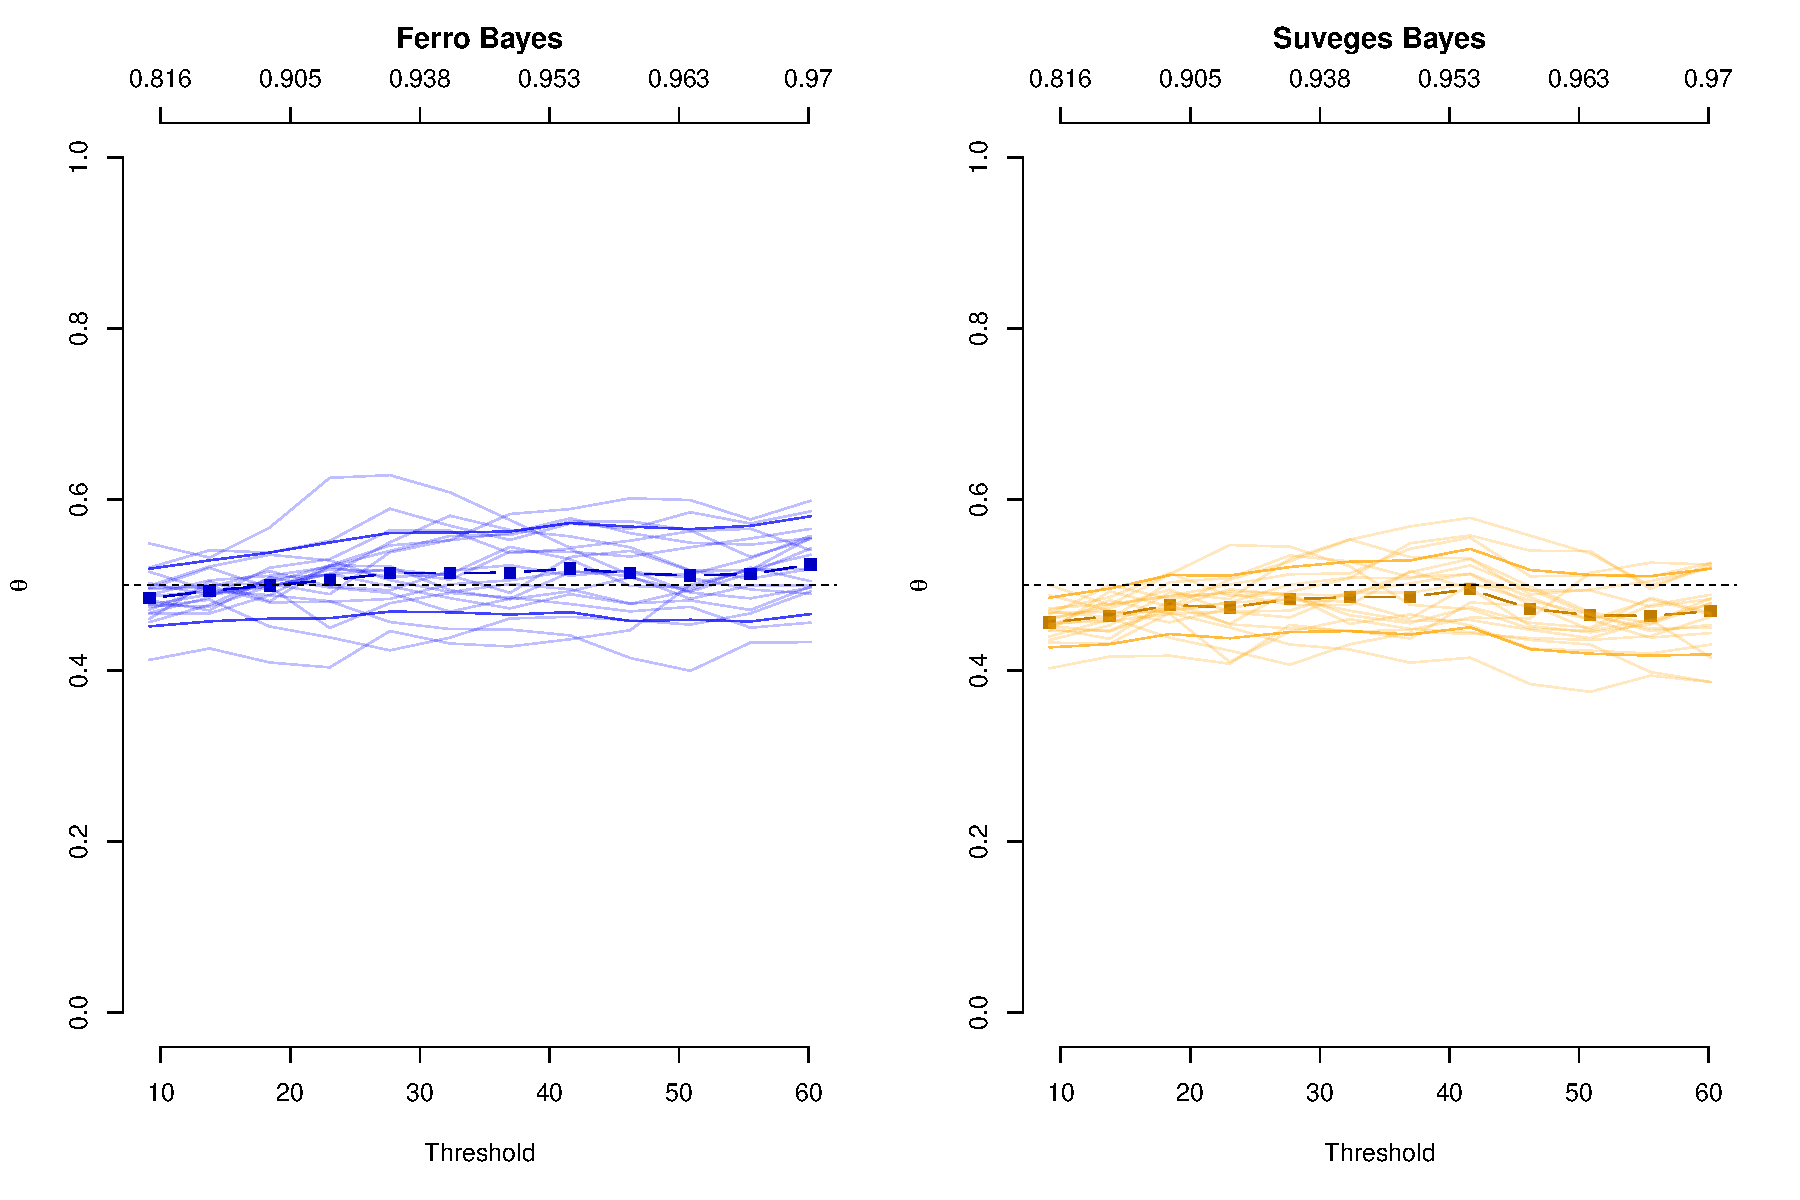
\includegraphics[width=5.5in, height=2.45in]{../extremal_comparison/figs/sim_frechet_hier_50_1000_20.pdf}
\caption{$\theta=0.50$, $n=1000$, $R=20$}
\end{center}
\end{figure}





\newpage

\begin{figure}
\begin{center}
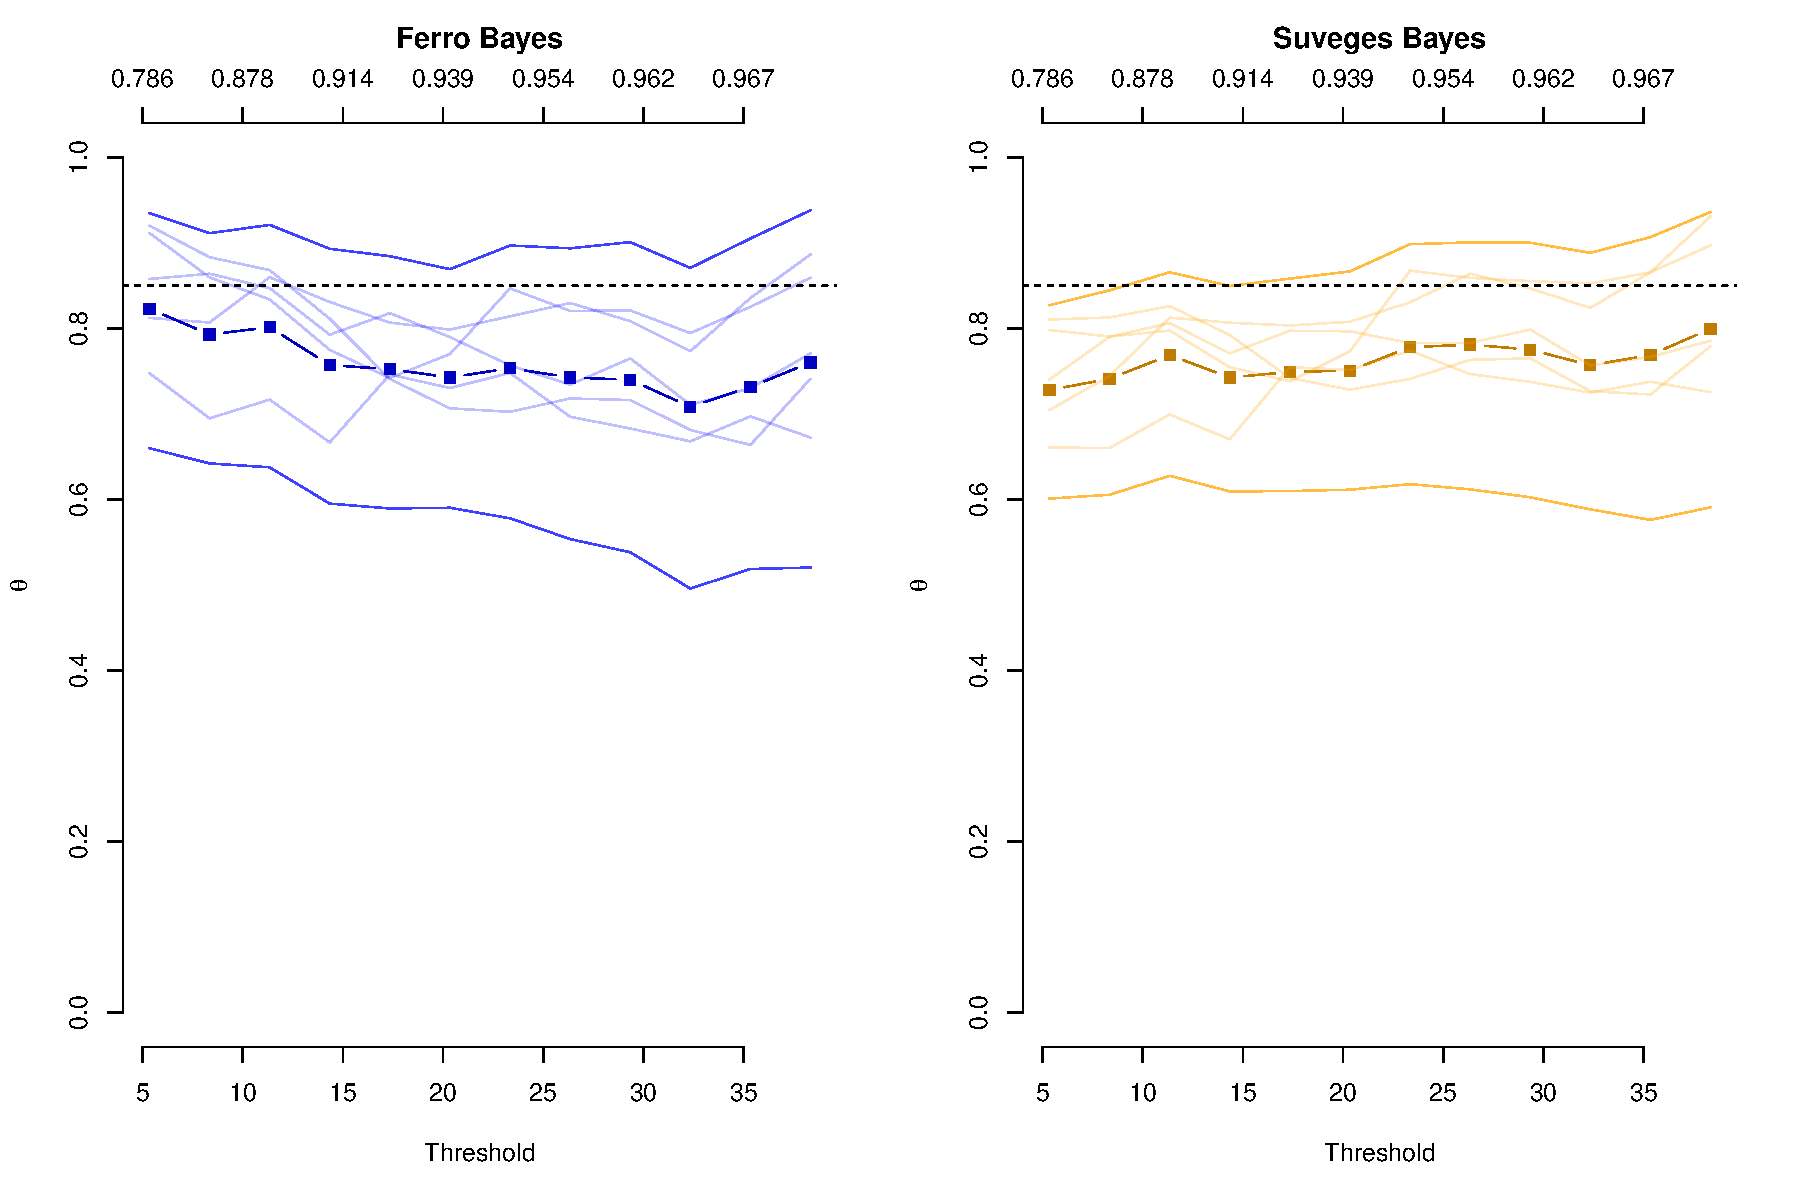
\includegraphics[width=5.5in, height=2.45in]{../extremal_comparison/figs/sim_frechet_hier_85_250_5.pdf}
\caption{$\theta=0.85$, $n=250$, $R=5$}
\end{center}
\end{figure}

\begin{figure}
\begin{center}
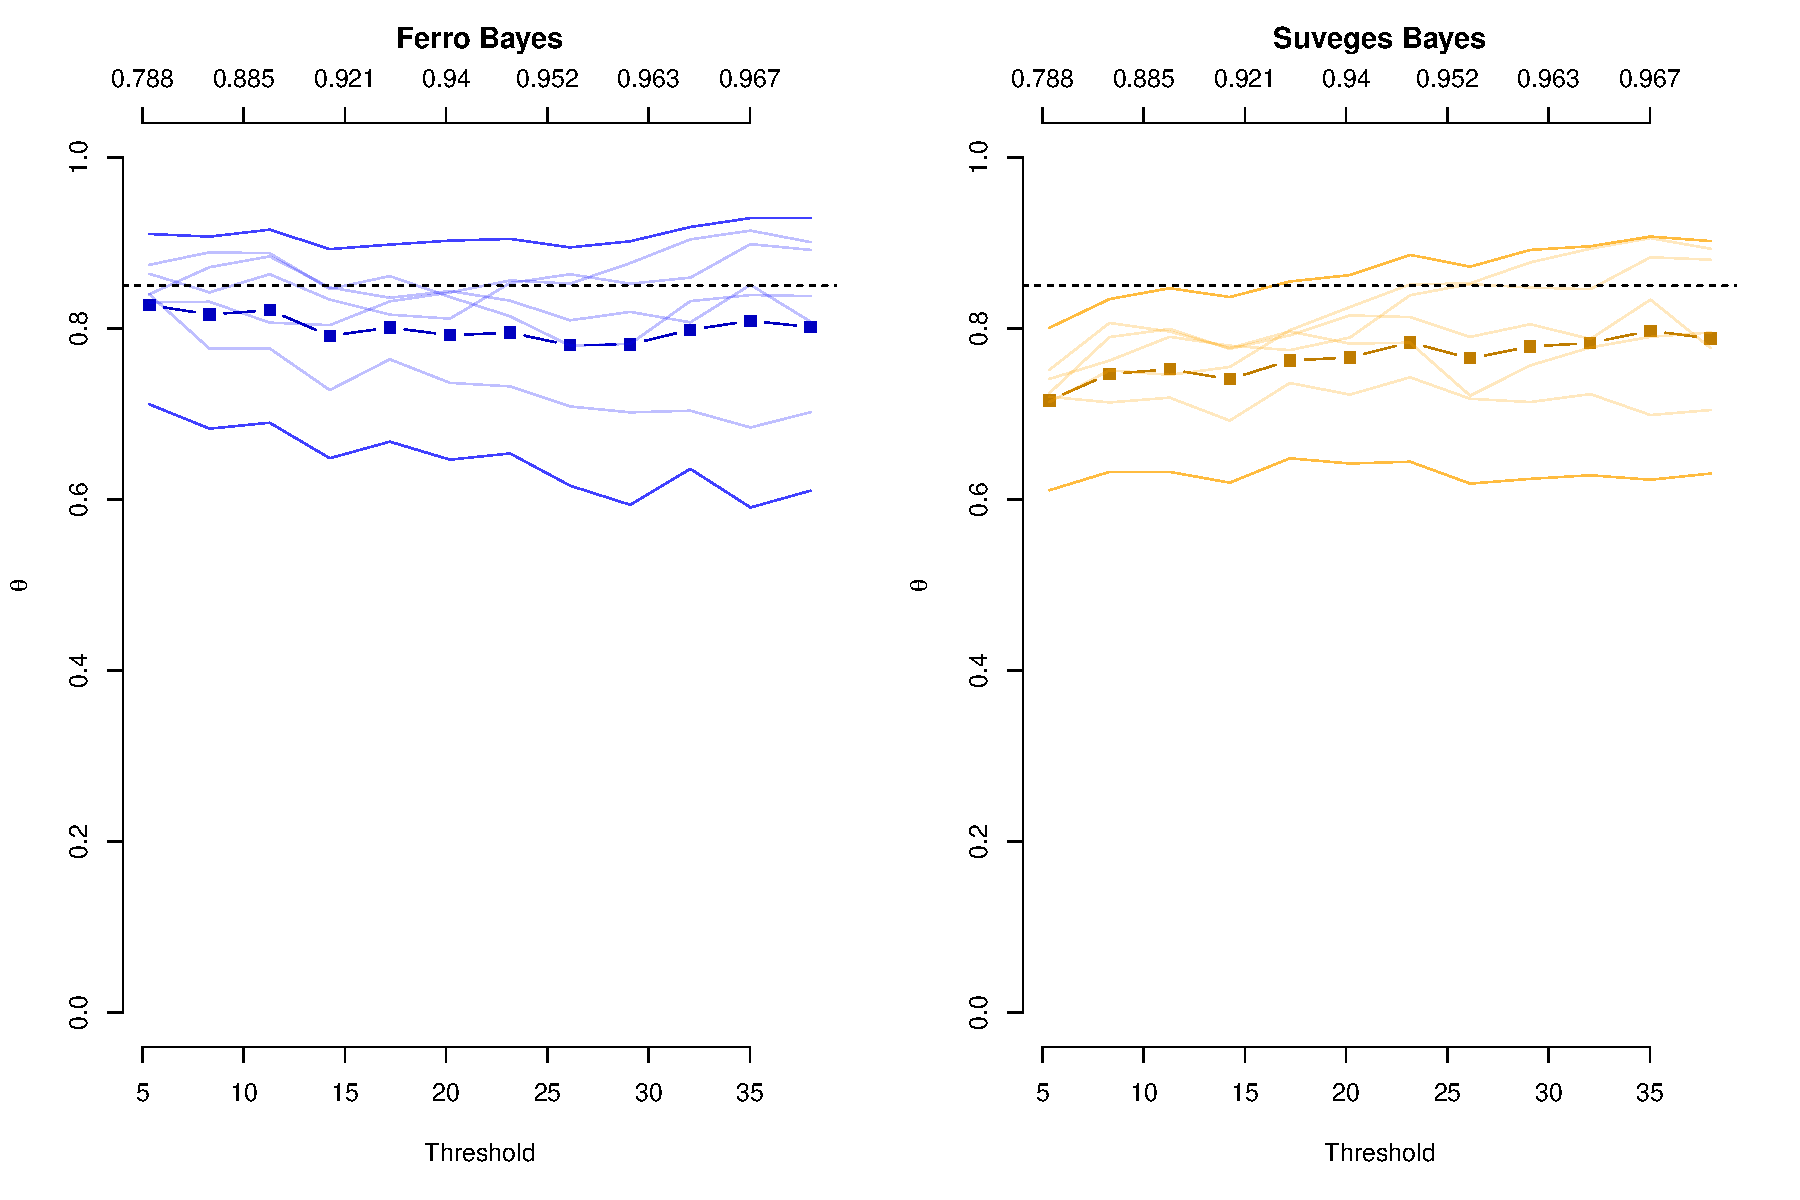
\includegraphics[width=5.5in, height=2.45in]{../extremal_comparison/figs/sim_frechet_hier_85_500_5.pdf}
\caption{$\theta=0.85$, $n=500$, $R=5$}
\end{center}
\end{figure}

\begin{figure}
\begin{center}
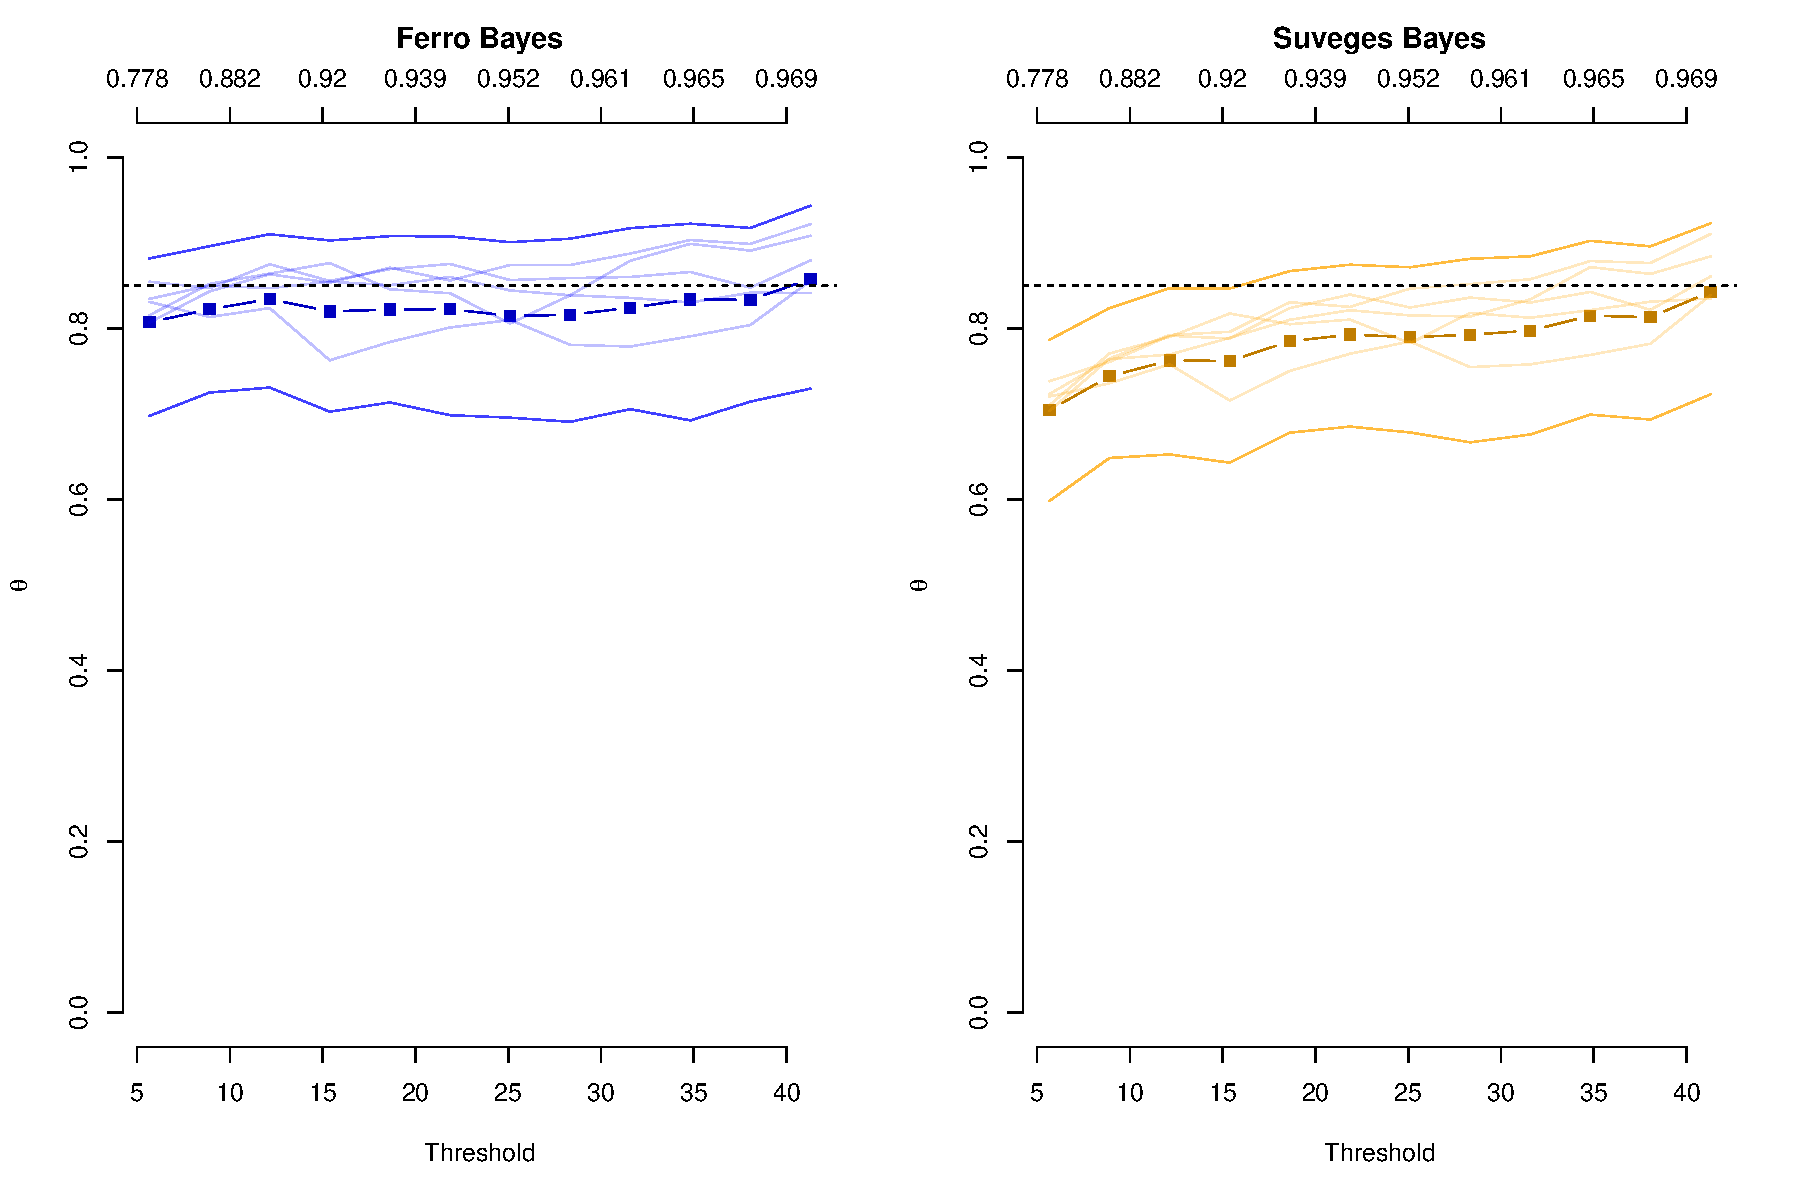
\includegraphics[width=5.5in, height=2.45in]{../extremal_comparison/figs/sim_frechet_hier_85_1000_5.pdf}
\caption{$\theta=0.85$, $n=1000$, $R=5$}
\end{center}
\end{figure}

\newpage

\begin{figure}
\begin{center}
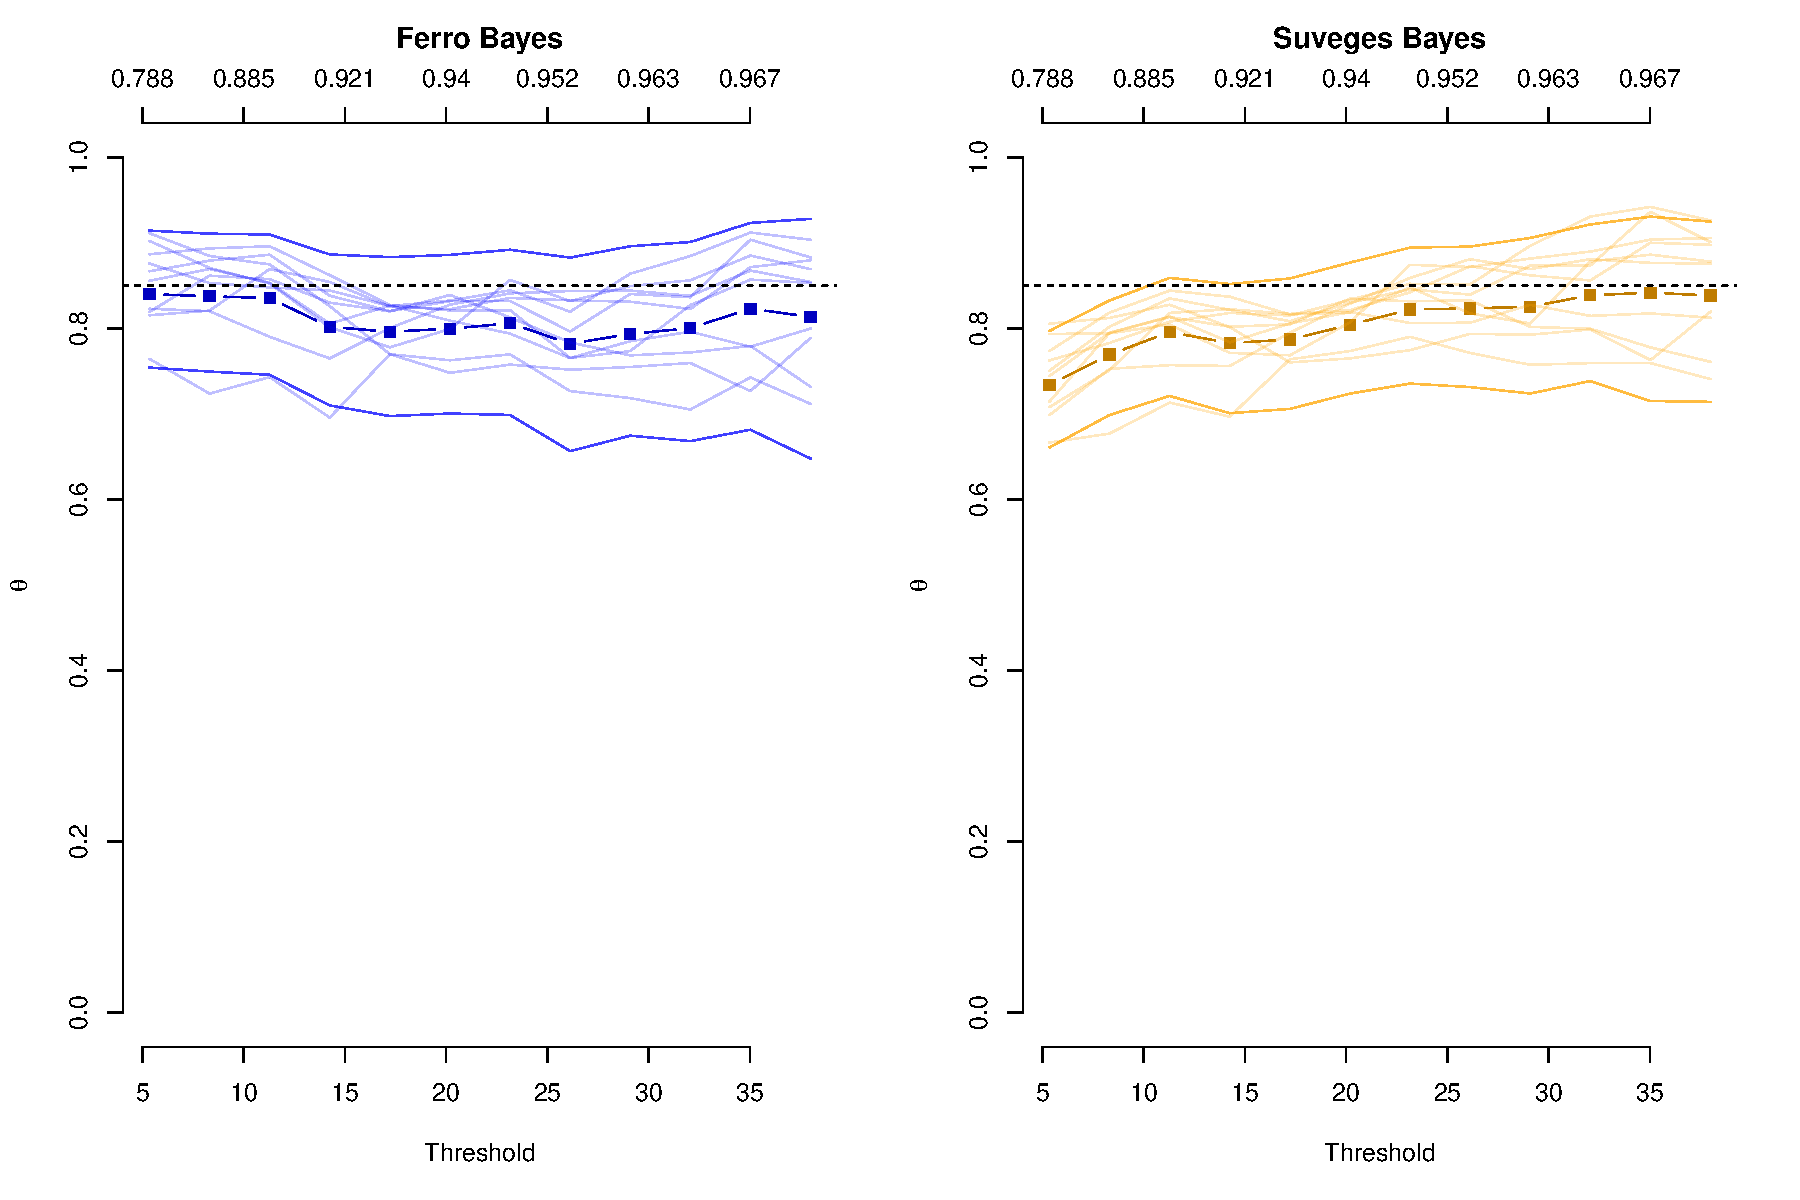
\includegraphics[width=5.5in, height=2.45in]{../extremal_comparison/figs/sim_frechet_hier_85_250_10.pdf}
\caption{$\theta=0.85$, $n=250$, $R=10$}
\end{center}
\end{figure}

\begin{figure}
\begin{center}
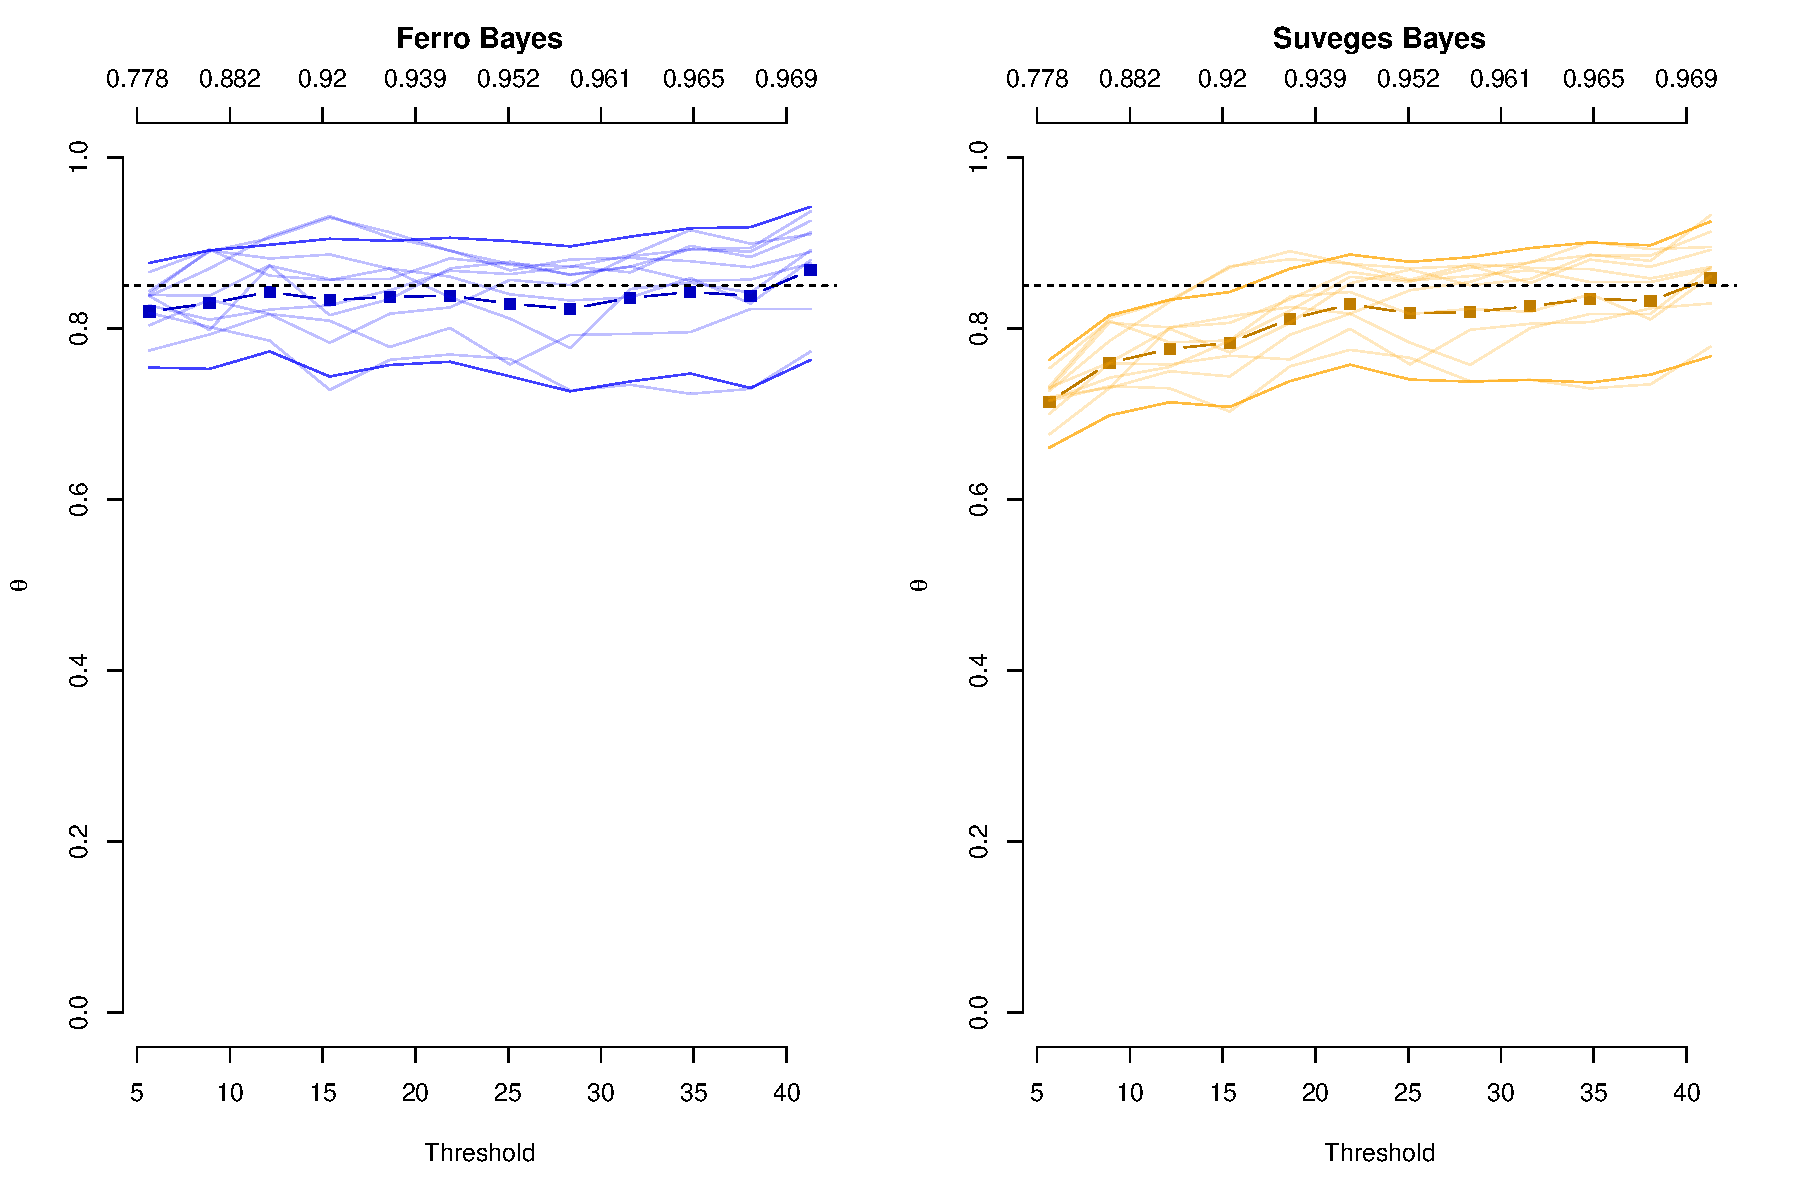
\includegraphics[width=5.5in, height=2.45in]{../extremal_comparison/figs/sim_frechet_hier_85_500_10.pdf}
\caption{$\theta=0.85$, $n=500$, $R=10$}
\end{center}
\end{figure}

\begin{figure}
\begin{center}
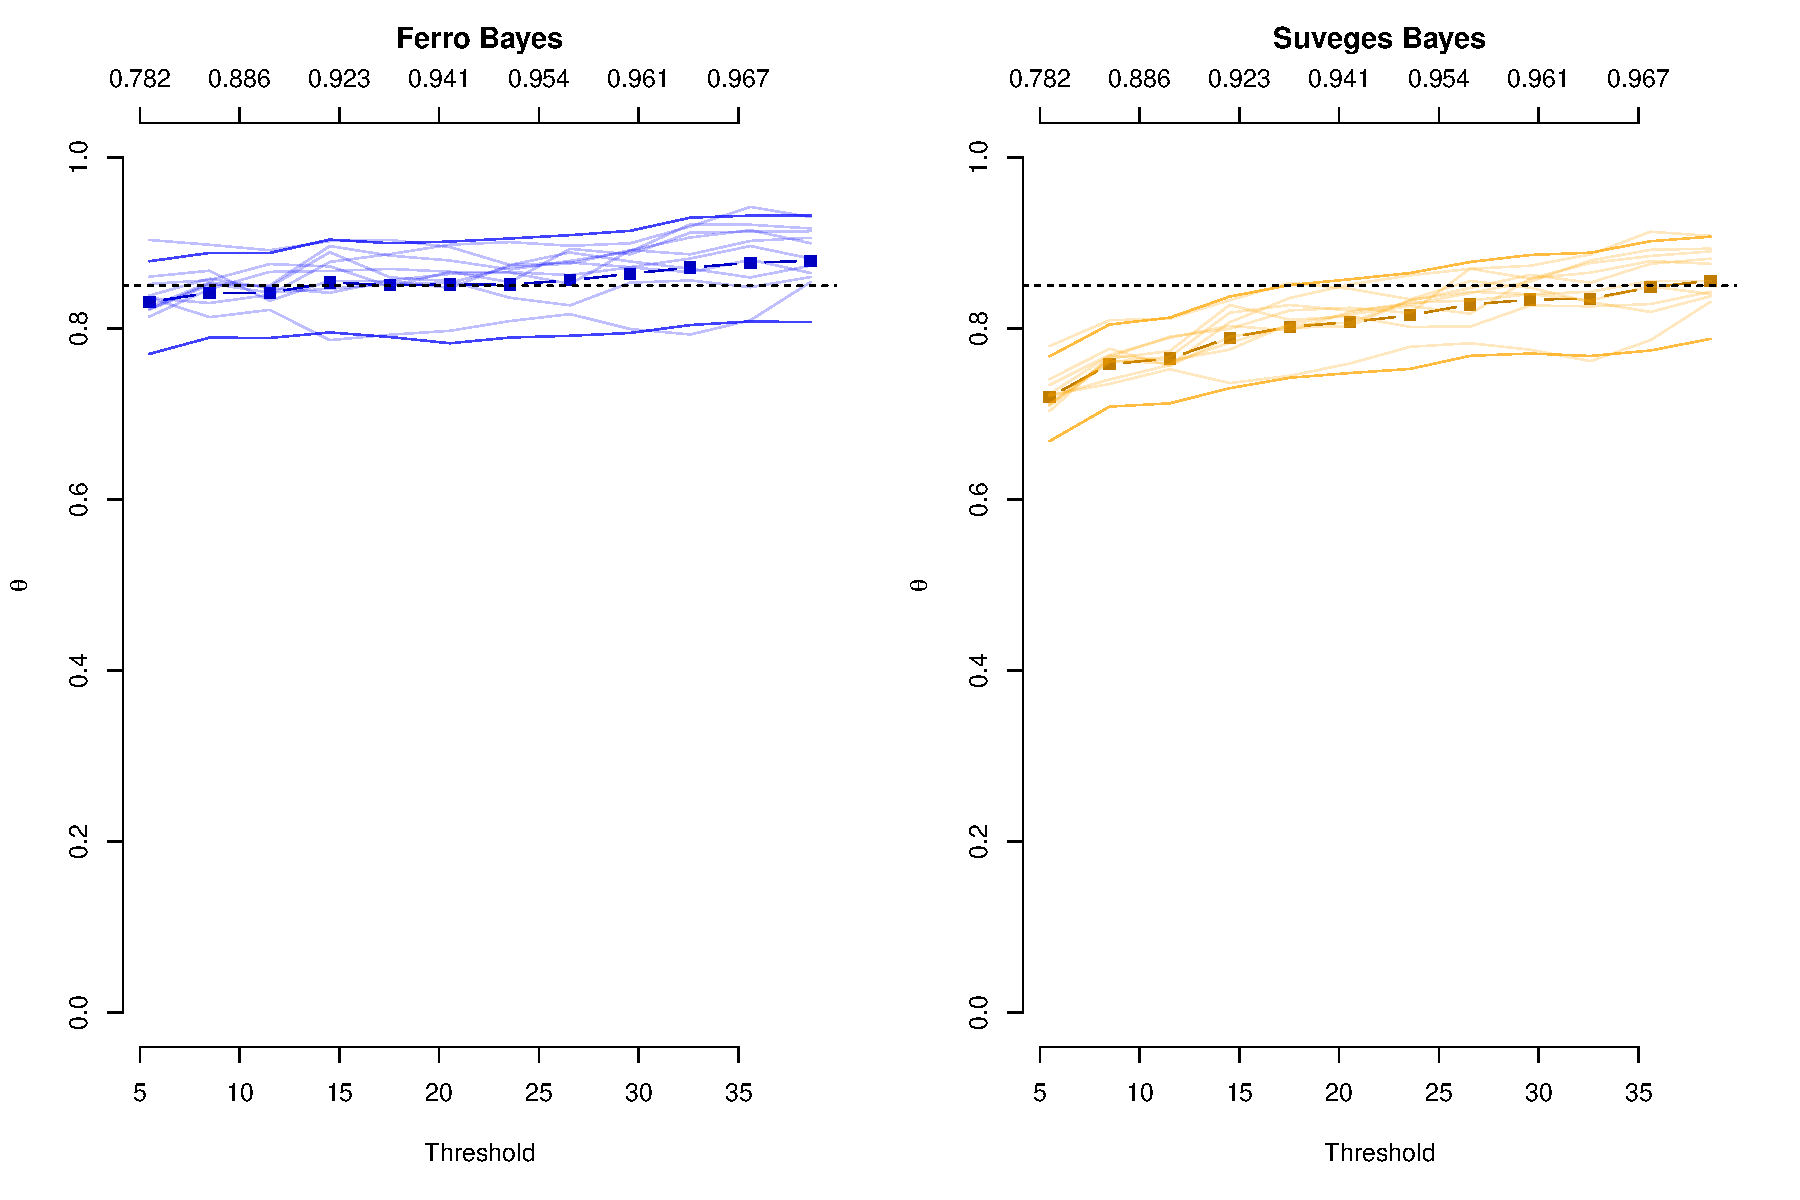
\includegraphics[width=5.5in, height=2.45in]{../extremal_comparison/figs/sim_frechet_hier_85_1000_10.pdf}
\caption{$\theta=0.85$, $n=1000$, $R=10$}
\end{center}
\end{figure}

\newpage

\begin{figure}
\begin{center}
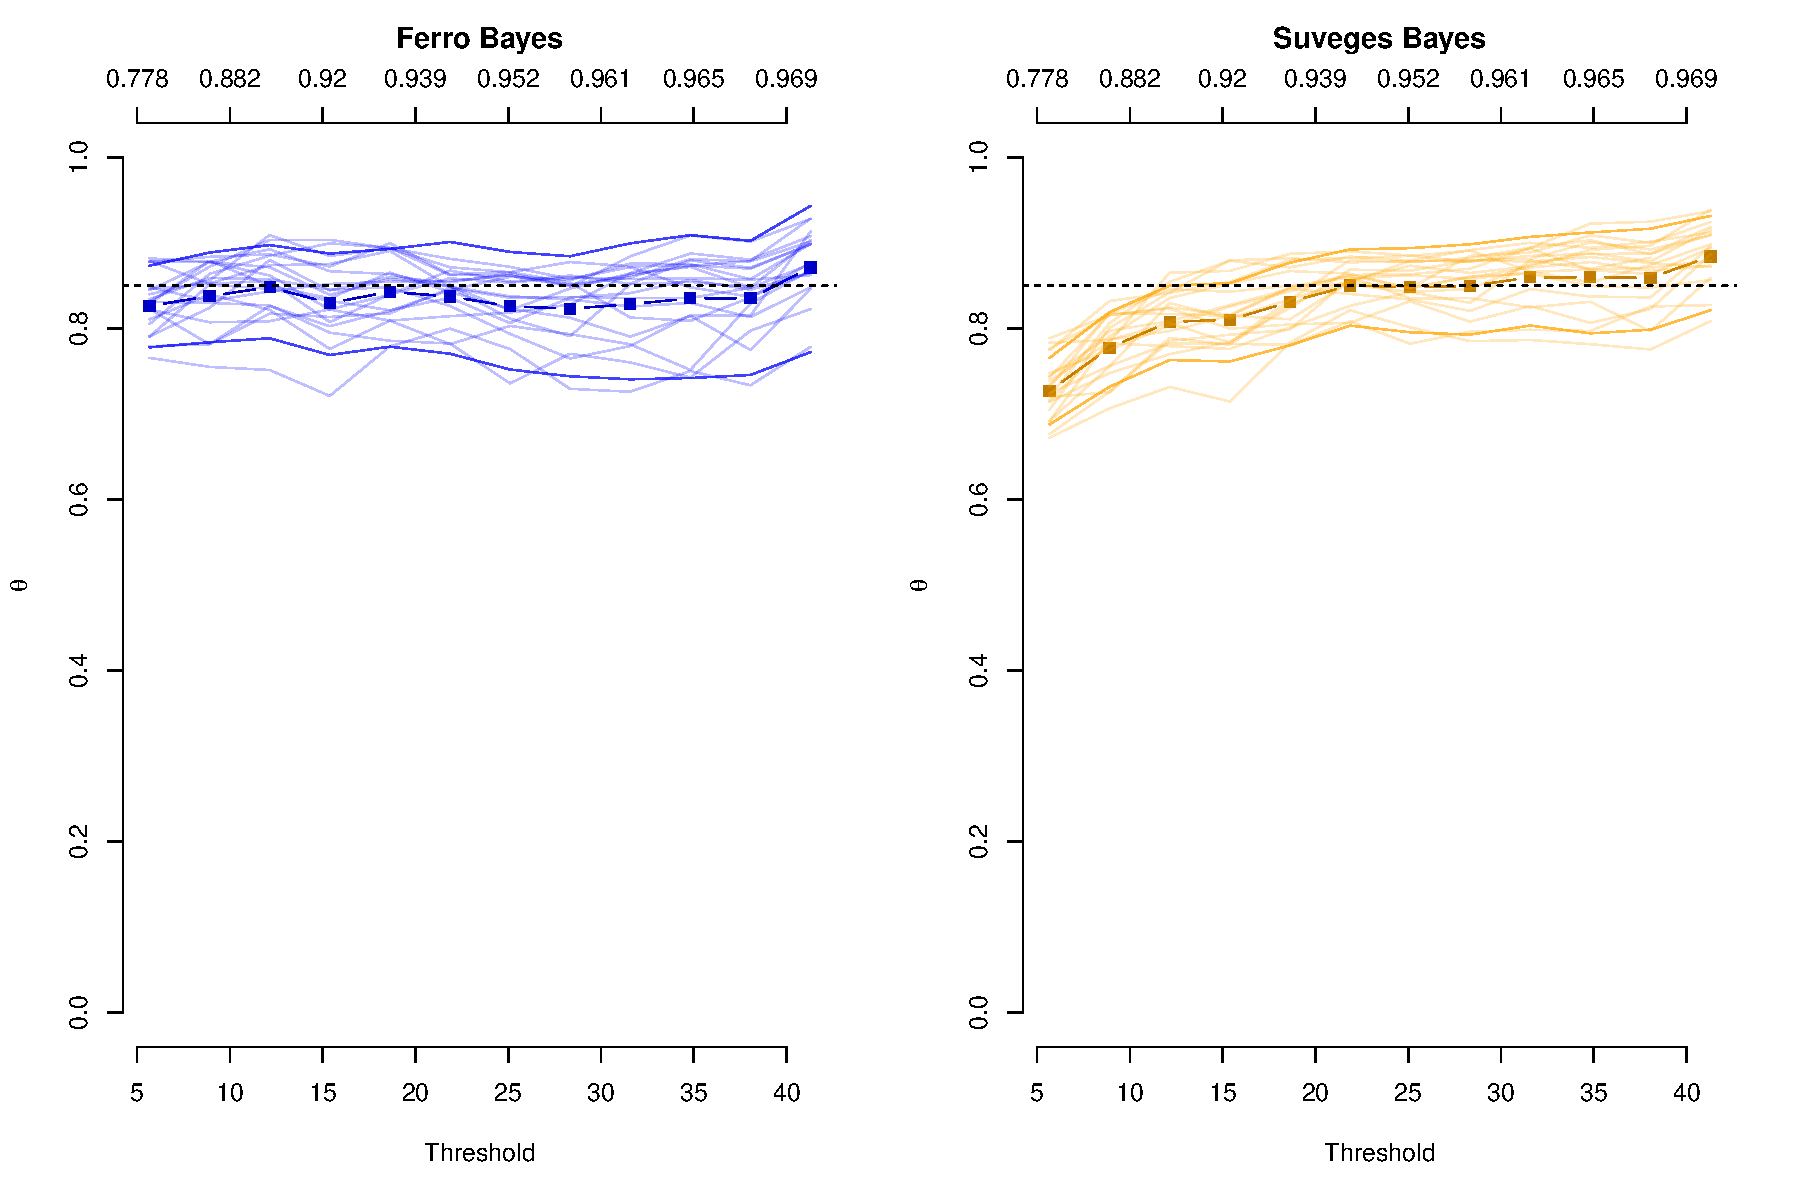
\includegraphics[width=5.5in, height=2.45in]{../extremal_comparison/figs/sim_frechet_hier_85_250_20.pdf}
\caption{$\theta=0.85$, $n=250$, $R=20$}
\end{center}
\end{figure}

\begin{figure}
\begin{center}
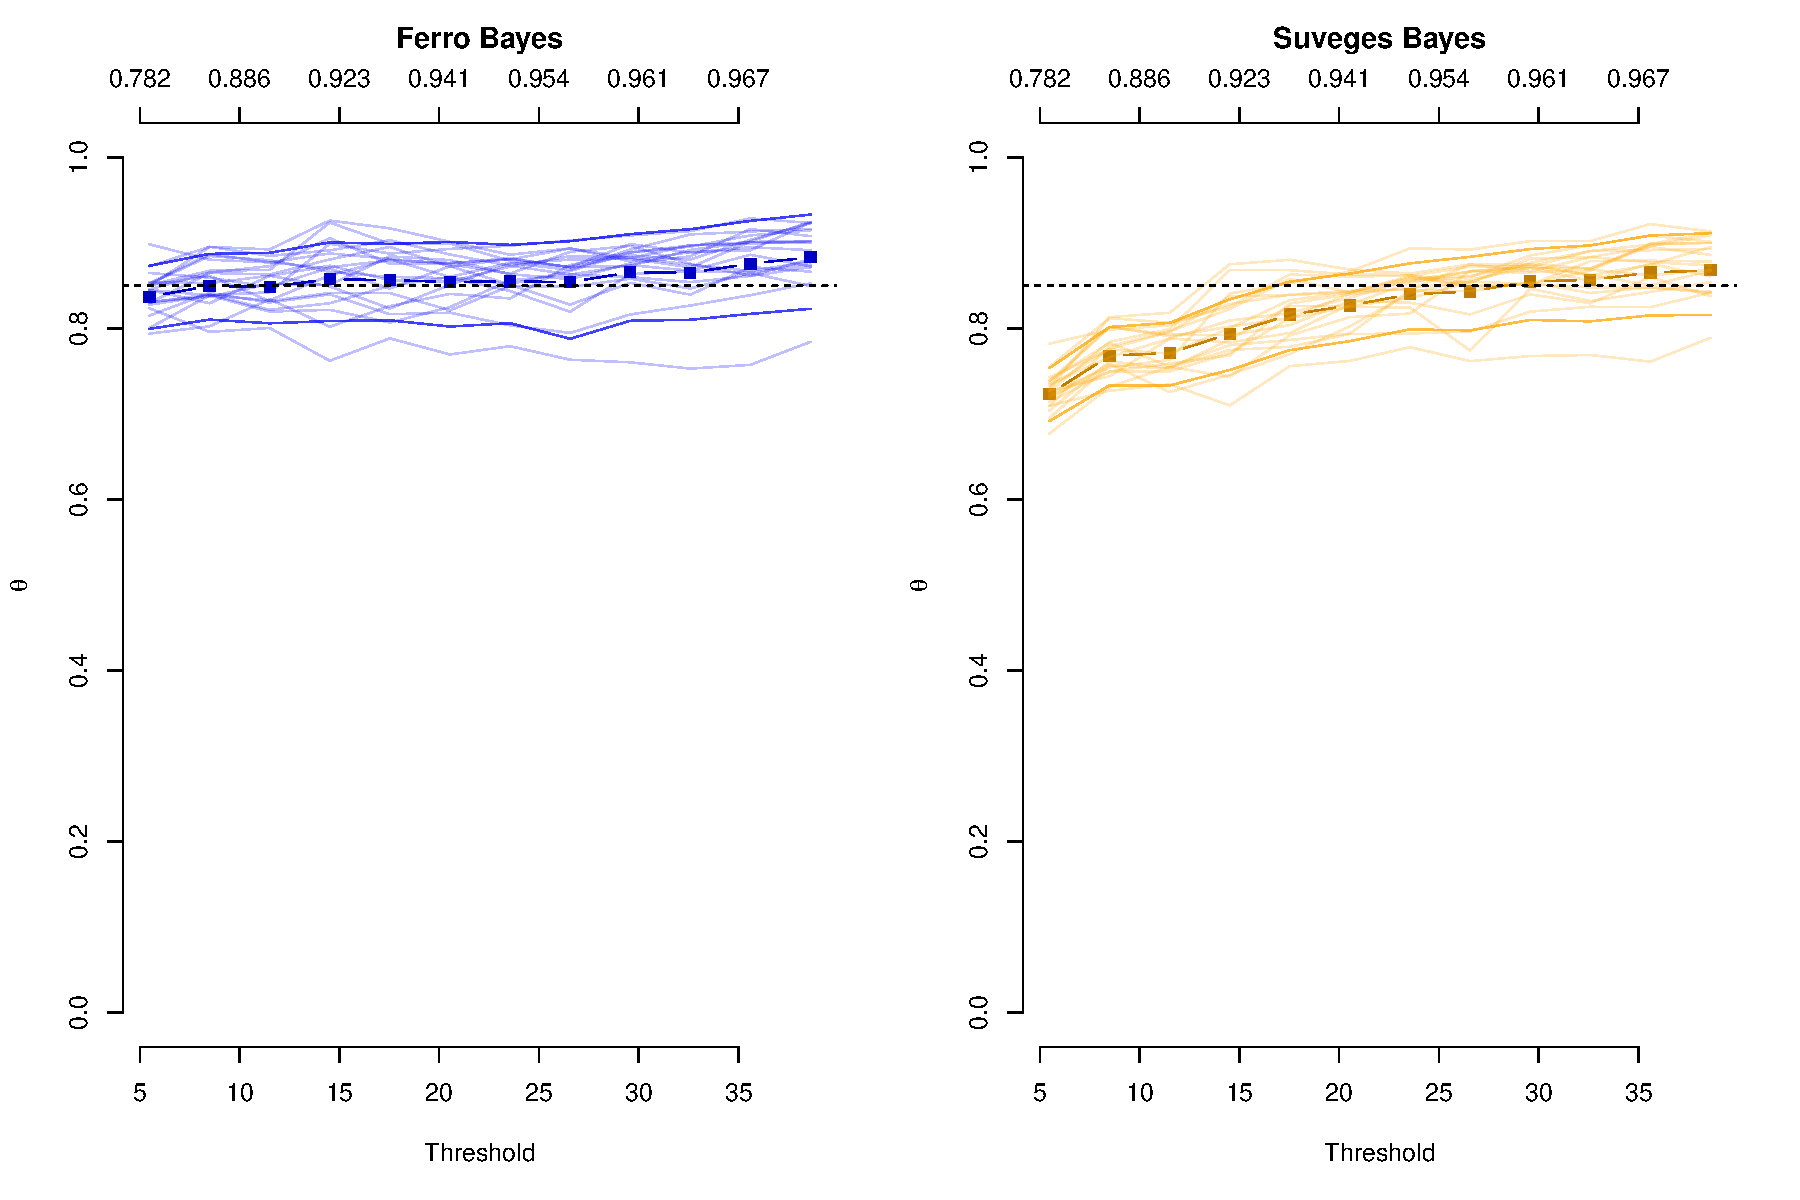
\includegraphics[width=5.5in, height=2.45in]{../extremal_comparison/figs/sim_frechet_hier_85_500_20.pdf}
\caption{$\theta=0.85$, $n=500$, $R=20$}
\end{center}
\end{figure}

\begin{figure}
\begin{center}
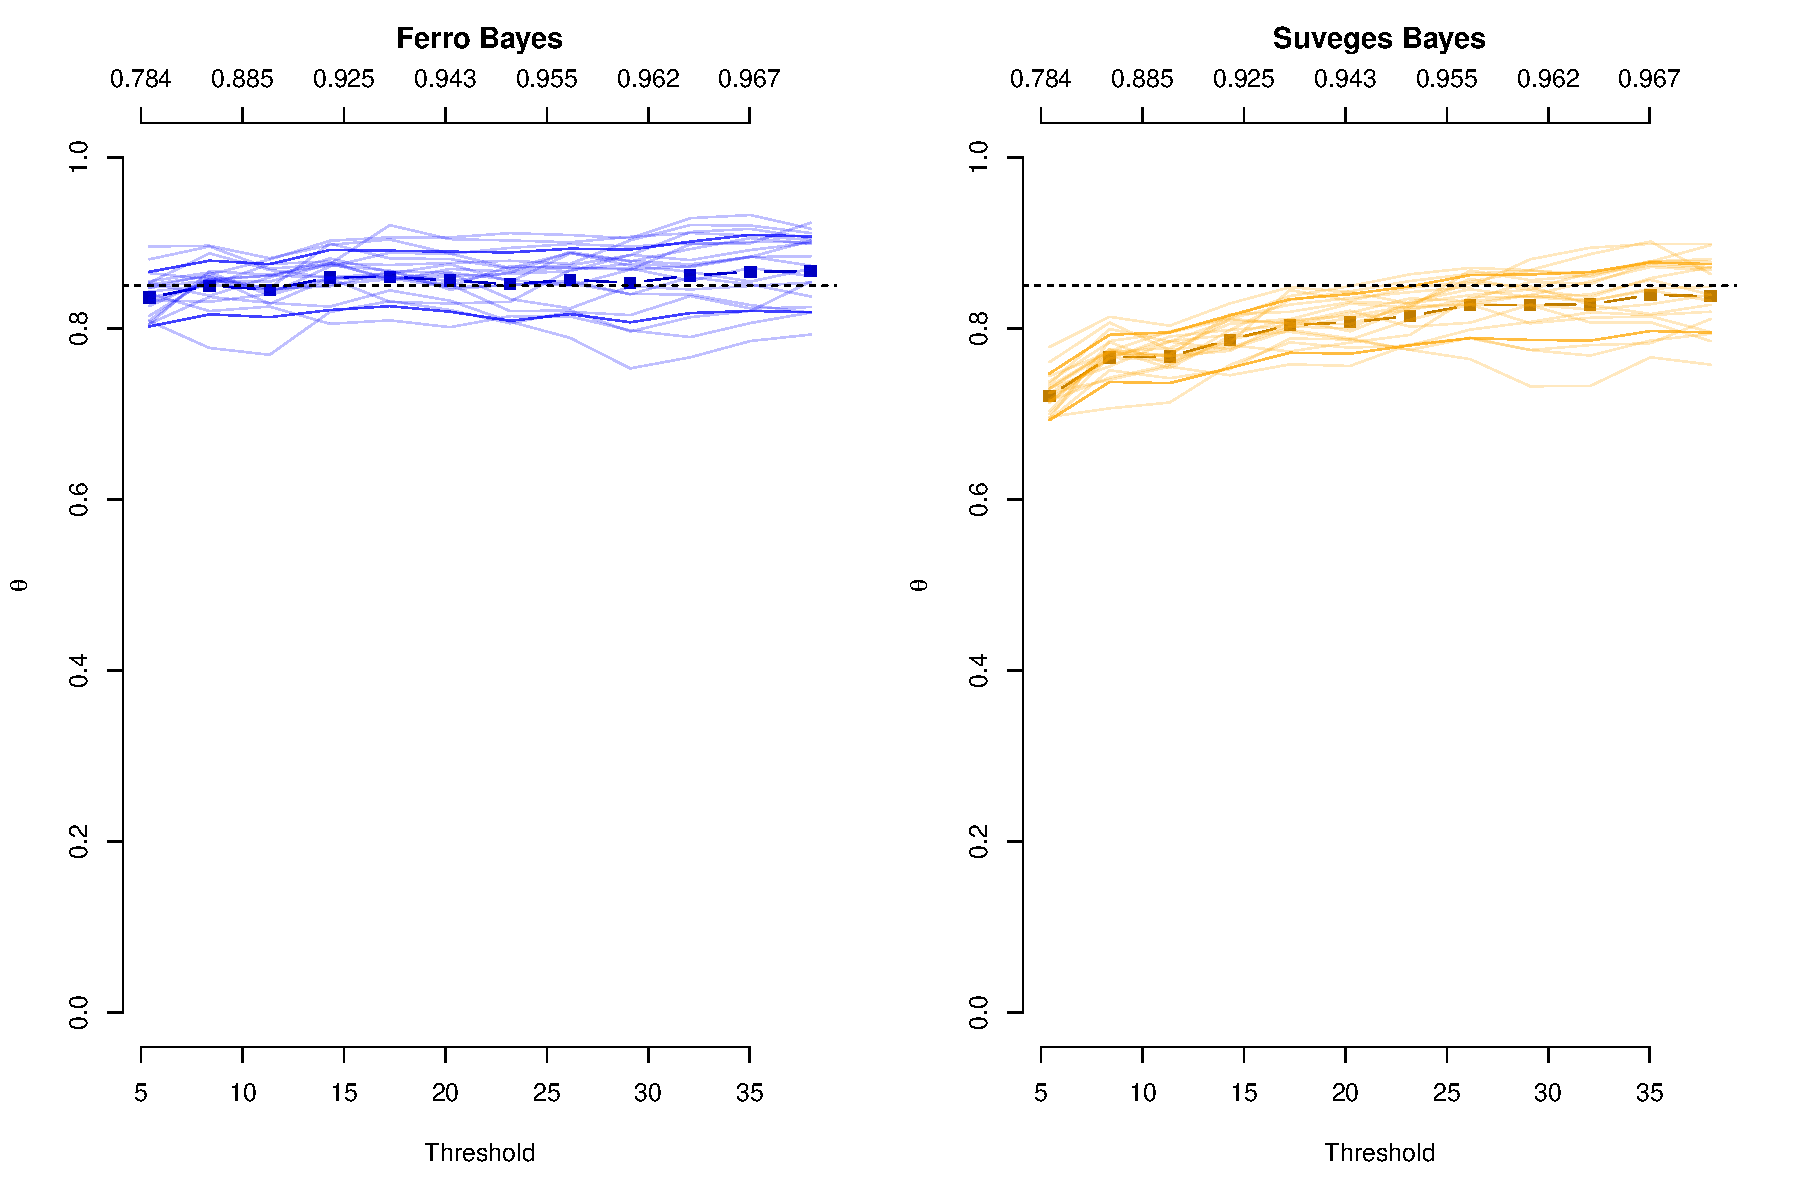
\includegraphics[width=5.5in, height=2.45in]{../extremal_comparison/figs/sim_frechet_hier_85_1000_20.pdf}
\caption{$\theta=0.85$, $n=1000$, $R=20$}
\end{center}
\end{figure}


\end{document}
